% !TeX program = xelatex
% 编码：UTF-8。建议使用 XeLaTeX 编译两次，以生成目录与交叉引用。
% 本文件使用同目录的《空间转录组学_CS_AI入门_讲义_配图》文件夹；无需 .bib 文件。
% 依据同目录《空间转录组学_CS_AI入门.pdf》整理。
% 保留原文 17 章的顺序、主要解释、类比、教学数据与参考来源。
% 新增与学术汇报相同的10幅教学配图；出处与许可随图标注。
\documentclass[UTF8,a4paper,11pt,fontset=fandol]{ctexart}

\usepackage[margin=2.35cm,headheight=23pt]{geometry}
\usepackage{amsmath,amssymb}
\usepackage{booktabs,tabularx,longtable,array}
\usepackage{graphicx}
\usepackage[table]{xcolor}
\usepackage{tcolorbox}
\tcbuselibrary{breakable}
\usepackage{tikz}
\usetikzlibrary{arrows.meta,positioning,calc}
\usepackage{enumitem}
\usepackage{fancyhdr}
\usepackage{caption}
\usepackage{xurl}
\usepackage[unicode,colorlinks=true]{hyperref}
\pdfstringdefDisableCommands{\def\quad{ }}
\hypersetup{
  pdftitle={空间转录组学入门：从细胞、DNA 和蛋白质到 CS 数据与科研问题},
  pdfsubject={面向计算机与人工智能专业本科生和研究生的入门讲义}}

% 学术讲义配色：深蓝标题、青色次级标题、浅蓝表格与提示框。
\definecolor{accent}{HTML}{244C6A}
\definecolor{tealaccent}{HTML}{286D77}
\definecolor{lightblue}{HTML}{EFF4F8}
\definecolor{tealwash}{HTML}{EDF5F4}
\definecolor{tablehead}{HTML}{DAE7F0}
\definecolor{muted}{HTML}{607384}
\definecolor{bodytext}{HTML}{24323D}
\hypersetup{linkcolor=accent,citecolor=tealaccent,urlcolor=tealaccent}
\pagestyle{fancy}
\fancyhf{}
\fancyhead[L]{\small\color{accent}AI4Science 入门资料\quad /\quad 空间转录组学}
\fancyhead[R]{\small\color{tealaccent}Auutuumn}
\fancyfoot[L]{\small\color{muted}从生物学概念到计算与科研}
\fancyfoot[R]{\small\color{accent}\thepage}
\renewcommand{\headrulewidth}{0.4pt}
\renewcommand{\headrule}{\hbox to\headwidth{\color{accent!45}\leaders\hrule height\headrulewidth\hfill}}
\setlength{\parindent}{2em}
\setlength{\parskip}{0.30em}
\linespread{1.12}
\setlength{\emergencystretch}{2em}
\renewcommand{\arraystretch}{1.3}
\setlength{\tabcolsep}{6pt}
\setlist{nosep,leftmargin=2em,topsep=0.4em}
\setlength{\intextsep}{9pt}
\captionsetup{skip=6pt,font={small,color=muted},labelfont={bf,color=accent},labelsep=quad}
\ctexset{
  section={format=\Large\bfseries\color{accent},beforeskip=0.5em,afterskip=0.7em},
  subsection={format=\normalsize\bfseries\color{tealaccent},beforeskip=0.6em,afterskip=0.2em}}
% 编号及目录均到 1.1 层级；各部分之间保留第 1--17 章的连续编号。
\setcounter{secnumdepth}{2}
\setcounter{tocdepth}{2}
\renewcommand{\thesubsection}{\thesection.\arabic{subsection}}
\newcolumntype{Y}{>{\raggedright\arraybackslash}X}
\newcommand{\term}[2]{{\color{accent}\textbf{#1}}（#2）}
\tcbset{learningstyle/.style={breakable,boxrule=0.4pt,arc=1mm,
  colback=lightblue,colframe=accent!45,colbacktitle=tablehead,
  coltitle=accent,fonttitle=\bfseries,left=3mm,right=3mm,
  top=2mm,bottom=2mm,before skip=0.8em,after skip=0.5em}}
\newcommand{\takeaway}[1]{\begin{tcolorbox}[learningstyle,title=本章要记住]#1\end{tcolorbox}}
\newcommand{\checkpoint}[1]{\begin{tcolorbox}[learningstyle,title=理解检查,
  colback=tealwash,colbacktitle=tealaccent!12,colframe=tealaccent!45,
  coltitle=tealaccent]#1\end{tcolorbox}}
\newcommand{\chapterstart}[1]{\clearpage\section{#1}}
\newcommand{\code}[1]{{\color{tealaccent}\texttt{#1}}}
% 部分页承担阅读导航；不改变章号，也不引入 1.1.1 级标题。
\newcommand{\partdivider}[3]{%
  \clearpage
  \refstepcounter{part}%
  \addcontentsline{toc}{part}{第\chinese{part}部分\quad #1}%
  \vspace*{0.16\textheight}
  \noindent{\large\color{tealaccent}第\chinese{part}部分}\par
  \vspace{0.6em}
  \noindent{\Huge\bfseries\color{accent}#1}\par
  \vspace{1.2em}
  \noindent{\color{tealaccent}\rule{0.2\linewidth}{2pt}}\par
  \vspace{1.2em}
  \noindent{\large\color{muted}#2}\par
  \vspace{1em}
  \begin{tcolorbox}[learningstyle,title=这一部分要理解什么]
    #3
  \end{tcolorbox}
  \vfill
  \noindent{\small\color{muted}空间转录组学入门\quad /\quad 学习路线}\par
}
\arrayrulecolor{accent!55}

\begin{document}
\color{bodytext}
% 在每页内容下方加淡色作者水印，不占用正文版面。
\AddToHook{shipout/background}{%
  \put(0pt,-\paperheight){%
    \parbox[b][\paperheight][c]{\paperwidth}{\centering
      \rotatebox{42}{\fontsize{34}{40}\selectfont\bfseries
        \color{accent!4.5!white}Auutuumn}}}%
}

\begin{center}
  {\LARGE\bfseries\color{accent}空间转录组学入门\par}
  \vspace{0.7em}
  {\large\color{tealaccent}从细胞、DNA 和蛋白质到 CS 数据与科研问题\par}
  \vspace{0.6em}
  {\color{muted}面向计算机与人工智能专业的本科生和研究生\par}
\end{center}
\noindent{\color{accent!50}\rule{\linewidth}{0.6pt}}

\noindent\textbf{适用读者：}有计算机或人工智能背景，但对生物学基本概念尚不熟悉的学生。本文从我们能想象的组织和细胞出发，逐步说明 RNA 怎样变成实验数据，再解释算法能用这些数据研究什么。不要求预先学过分子生物学；读到矩阵部分时，具备基本的线性代数和机器学习概念会有帮助。

\noindent\textbf{写作动机：}我的研究生学习领域涉及空间转录组学相关知识。在学习和研究过程中，我体会到，刚接触这一方向的同学往往需要先熟悉一些生物学概念，才能进一步理解实验数据和计算方法。因此，我整理了这份入门资料，希望把相关知识讲得更清楚一些，也帮助更多同学顺利迈出第一步。

读完后，我们应该能够用自己的话说明：空间转录组测什么、为什么要保留位置、矩阵的一行和一列代表什么，以及一个 AI 模型的输出如何成为有依据的科学结论。

\subsection*{先给脑中放一张简单的图}
一小块组织里有许多细胞。研究人员测量不同位置的 RNA，用这些分子信号了解细胞的身份和状态，再把信息放回组织地图。这就是后面所有内容的起点。RNA 是什么、为什么能提供线索，我们接下来慢慢解释。

\begin{center}
\rowcolors{2}{lightblue}{white}
\begin{tabularx}{\linewidth}{@{}l l Y@{}}
\toprule
\rowcolor{tablehead}
阶段 & 阅读内容 & 理解目标 \\
\midrule
先认识研究对象 & 第 1--5 章 & 细胞、DNA、基因、RNA、蛋白质和表达 \\
再理解测量方法 & 第 6--9 章 & 转录组、单细胞、空间信息与实验读数 \\
最后进入 CS 与科研 & 第 10--15 章 & 数据表示、分析流程、研究问题和验证 \\
遇到术语时回查 & 第 16--17 章 & 核心名词及来源 \\
\bottomrule
\end{tabularx}
\end{center}

\subsection*{贯穿全文的例子}
我们假设研究人员拿到一张肿瘤组织薄片，想了解“不同细胞在哪里，以及免疫细胞是否出现在肿瘤内部”。这是一个研究问题示例，不预设答案，也不凭细胞分布直接判断治疗效果。后面的计数和布局均为教学构造。

我们不需要一次读完。前五章能讲清楚，就已经补上了理解空间转录组最关键的基础。类比帮助建立直觉，但不能代替真实的分子与实验过程。



\clearpage
\tableofcontents

\partdivider{生物学基础}{第 1--5 章：从组织和细胞到基因表达}{%
  先认识研究对象，再认识细胞如何保存和使用信息。建立 DNA、基因、RNA、蛋白质与表达之间的联系，区分细胞类型和细胞状态，为理解实验读数做好准备。}

\chapterstart{先认识组织和细胞}
想象医生取出一小块组织，把它切成薄片，放在显微镜下。这张薄片并不是均匀的一团材料：里面有许多细胞，细胞之间还有支撑它们的物质。我们研究的“组织”，就是这样的结构。

\subsection{组织和细胞分别在哪一层}
\begin{center}
\rowcolors{2}{lightblue}{white}
\begin{tabularx}{\linewidth}{@{}l Y l@{}}
\toprule
\rowcolor{tablehead}
层次 & 简单解释 & 例子 \\
\midrule
人体 & 整个生命个体 & 一个人 \\
器官 & 多种组织共同承担一定功能的结构 & 心脏 \\
组织 & 细胞与周围材料形成的结构 & 心脏中的心肌组织 \\
细胞 & 人体结构和功能的基本单位 & 心肌细胞 \\
\bottomrule
\end{tabularx}
\end{center}

所以，我们可以先记住“人体 $\rightarrow$ 器官 $\rightarrow$ 组织 $\rightarrow$ 细胞”。组织比细胞大，但组织不仅仅是细胞的简单堆积，细胞之间的材料和排列也属于组织的一部分。\cite{nci-organ}

\subsection{细胞可以想象成一个微小的工作单位}
典型有核人体细胞外面有细胞膜，内部有细胞质和细胞核。细胞膜像边界；细胞质是内部许多活动发生的环境；细胞核保存着大部分 DNA。这里描述的是常见结构，人体也有成熟红细胞等例外，不需要用例外打断最初的理解。

细胞有不同分工。例如，上皮细胞构成身体表面或器官内壁等结构；免疫细胞参与防御；成纤维细胞参与组织支撑和修复。先认识这三类名字就够了，不必现在背全部细胞分类。


% BEGIN ADDED IMAGE nucleus
\begin{figure}[!htbp]\centering
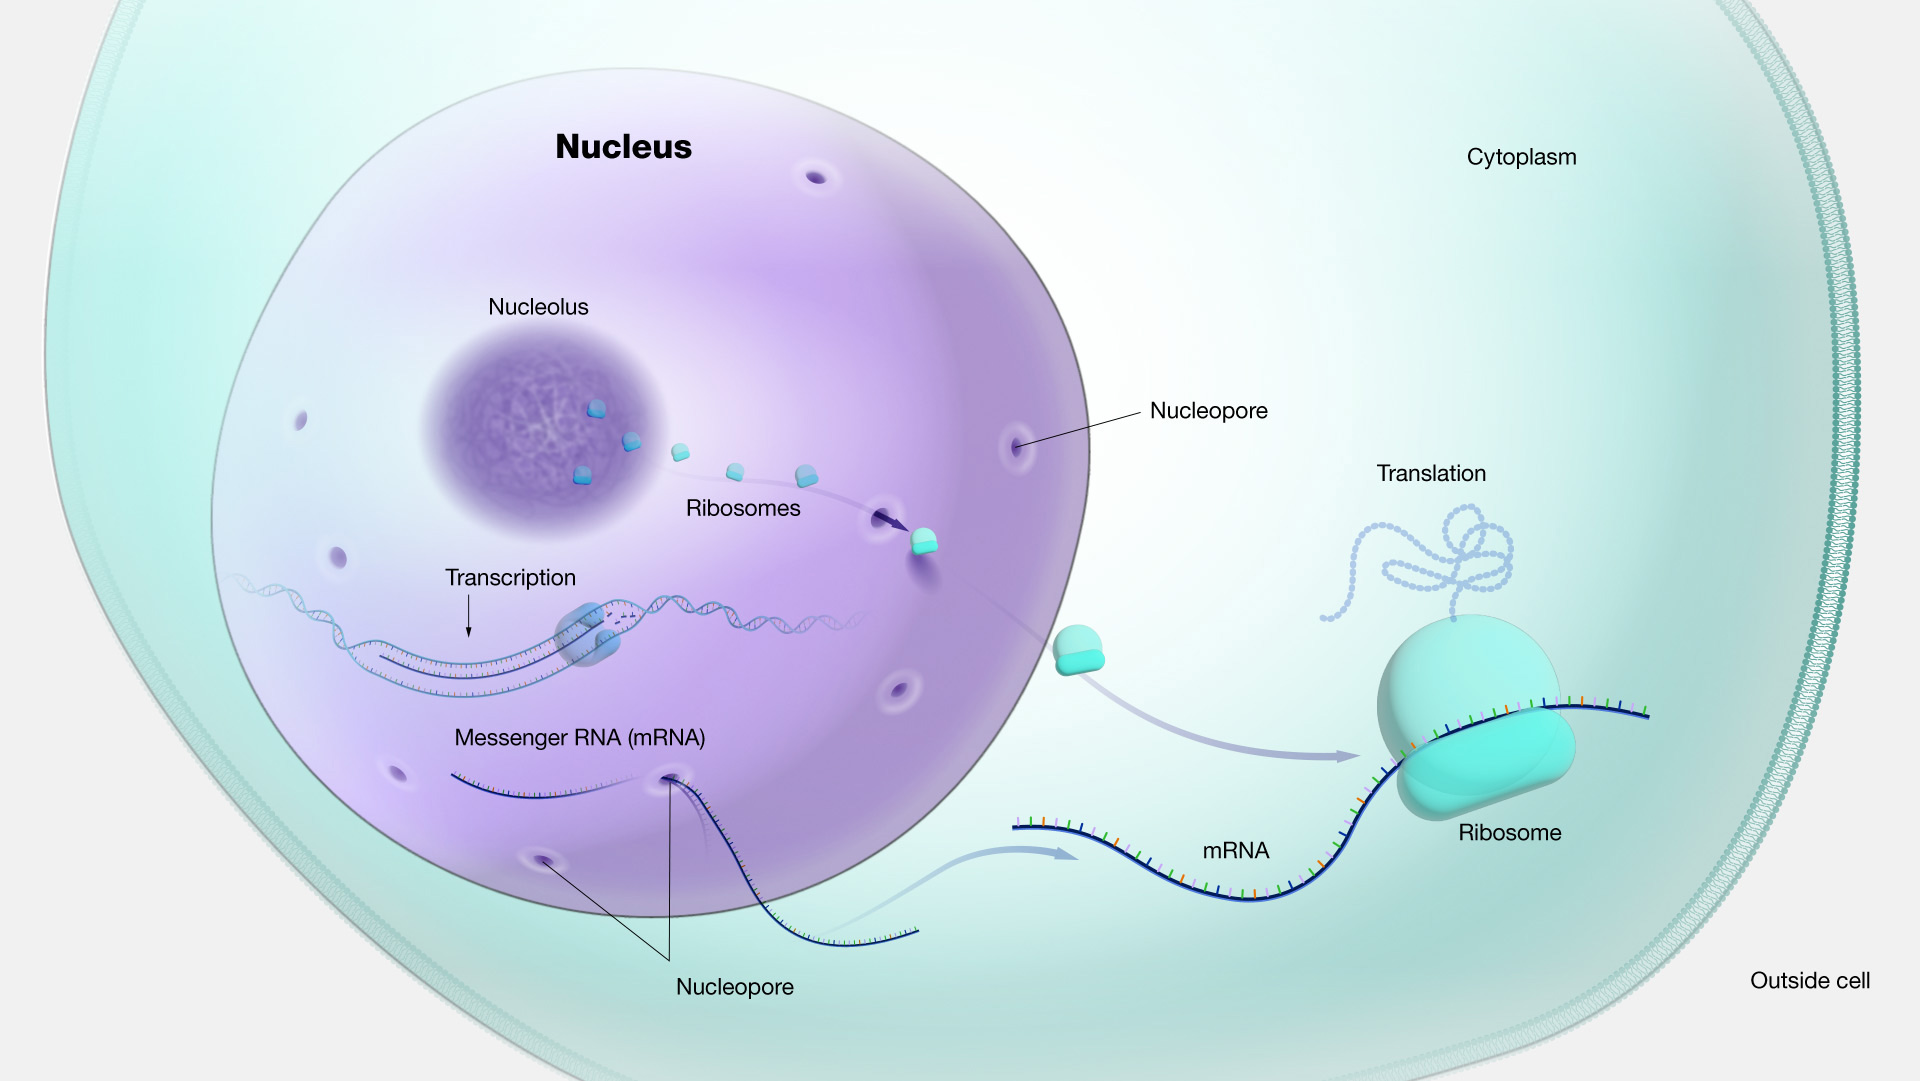
\includegraphics[width=.95\linewidth]{空间转录组学_CS_AI入门_讲义_配图/nucleus.jpg}
\caption{典型有核细胞的局部示意。紫色区域为细胞核（Nucleus），其外为细胞质（Cytoplasm），最外侧为细胞膜；核糖体参与蛋白质合成。先认识这些位置关系，图中的转录与翻译将在后文展开。示意颜色与尺寸用于教学，不是显微照片。}\label{fig:handout-nucleus}
\par\smallskip{\footnotesize\color{muted}\raggedright 图片：\href{https://www.genome.gov/genetics-glossary/Nucleus}{NHGRI}；许可：\href{https://www.genome.gov/about-nhgri/Policies-Guidance/Copyright}{Public domain}；原图等比缩放。\par}
\end{figure}
% END ADDED IMAGE nucleus

\subsection{为什么显微镜照片还不够}
照片能提供外形、排列和组织结构的线索，专家也能据此作出许多判断。但它不能直接给出所有细胞的分子状态。我们希望知道某个细胞是否在增殖、是否受到刺激，以及它属于哪类细胞；这时需要更多测量。


% BEGIN ADDED IMAGE histology
\begin{figure}[!htbp]\centering
\begin{minipage}[c]{.42\linewidth}\centering 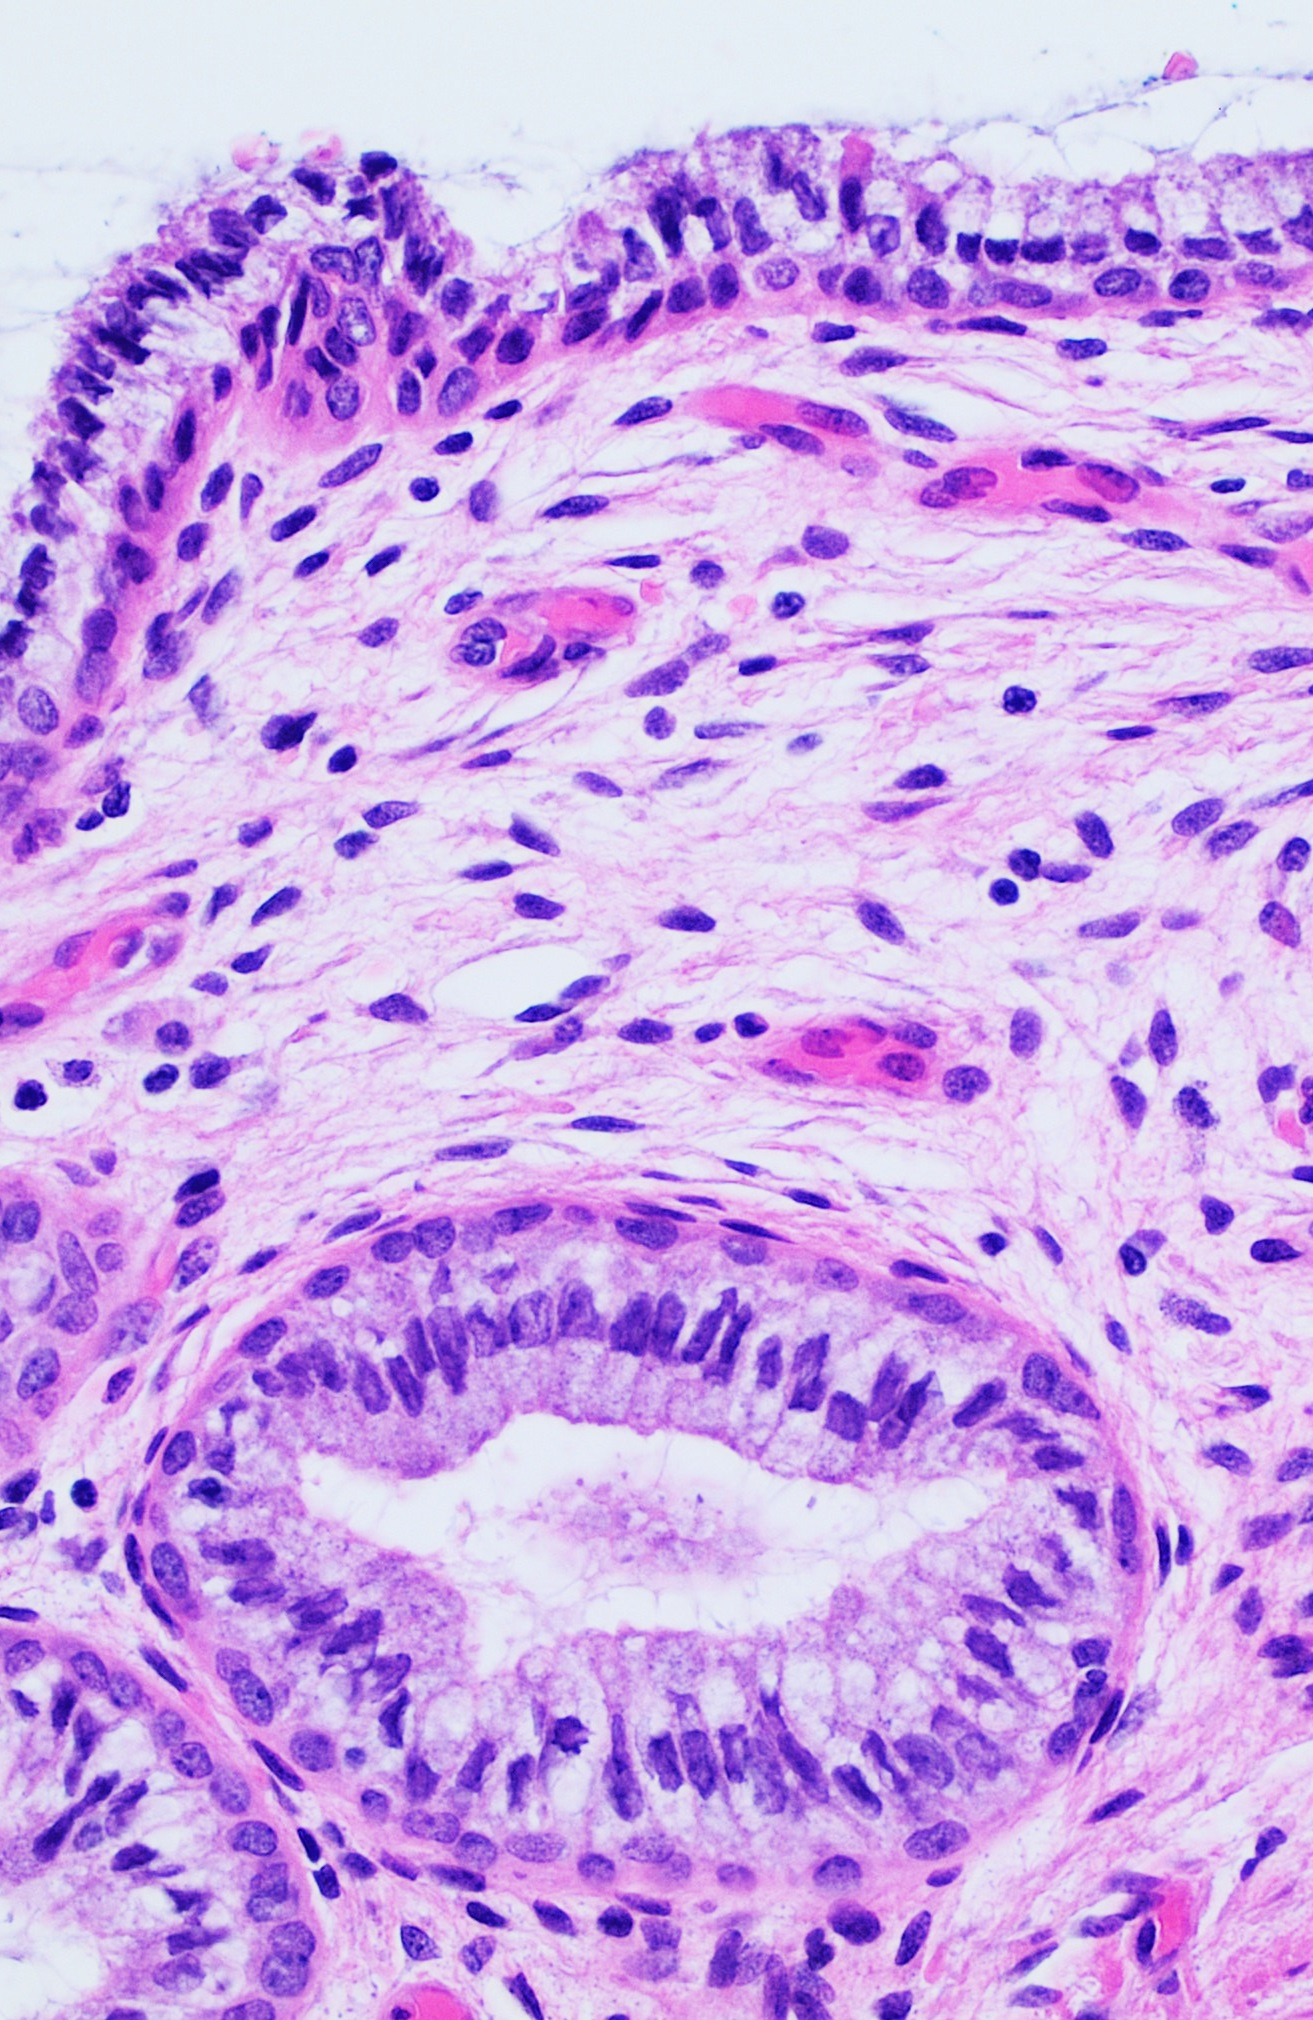
\includegraphics[width=.92\linewidth]{空间转录组学_CS_AI入门_讲义_配图/histology.jpg}\end{minipage}\hfill\begin{minipage}[c]{.53\linewidth}\small \textbf{先看组织的排列。}深紫色区域帮助观察细胞核的位置，图中还能看到表面上皮和下方的腺体结构。\par\medskip \textbf{再区分形态与分子测量。}组织照片有助于认识结构；若要知道哪些基因在这些位置表达，还需要相应的分子测量。\end{minipage}
\caption{真实的宫颈管组织显微图像，采用苏木精—伊红（H\&E）染色。它展示了形态与排列，但不能直接给出各位置的 RNA 表达；此图不是贯穿全文肿瘤案例的样本。}\label{fig:handout-histology}
\par\smallskip{\footnotesize\color{muted}\raggedright 图片：\href{https://commons.wikimedia.org/wiki/File:Histology_of_endocervix.jpg}{Mikael H\"aggstr\"om}；许可：\href{https://creativecommons.org/publicdomain/zero/1.0/}{CC0 1.0}；原图等比缩放。\par}
\end{figure}
% END ADDED IMAGE histology

回到肿瘤薄片：我们能看到一片组织，但还想知道其中哪些位置有免疫细胞。这就要进一步认识细胞里面保存和使用的信息。

\takeaway{组织里有细胞；细胞有不同分工；照片提供形态，分子测量提供另一类信息。}

\chapterstart{DNA 和基因究竟是什么}
\subsection{DNA 是保存遗传信息的分子}
DNA 是一种实际存在的分子，不是抽象概念。它的结构常画成双螺旋，像扭转的梯子。DNA 的序列可用 A、T、C、G 四种字母表示；这些字母代表不同的碱基，它们的排列承载遗传信息。\cite{nhgri-dna}

作为 CS 学生，我们可以把 DNA 序列先看成很长的字符串。但真实 DNA 是分子，它的包装方式和细胞中的环境也会影响信息如何被使用。字符串只是第一层表示。


% BEGIN ADDED IMAGE dna
\begin{figure}[!htbp]\centering
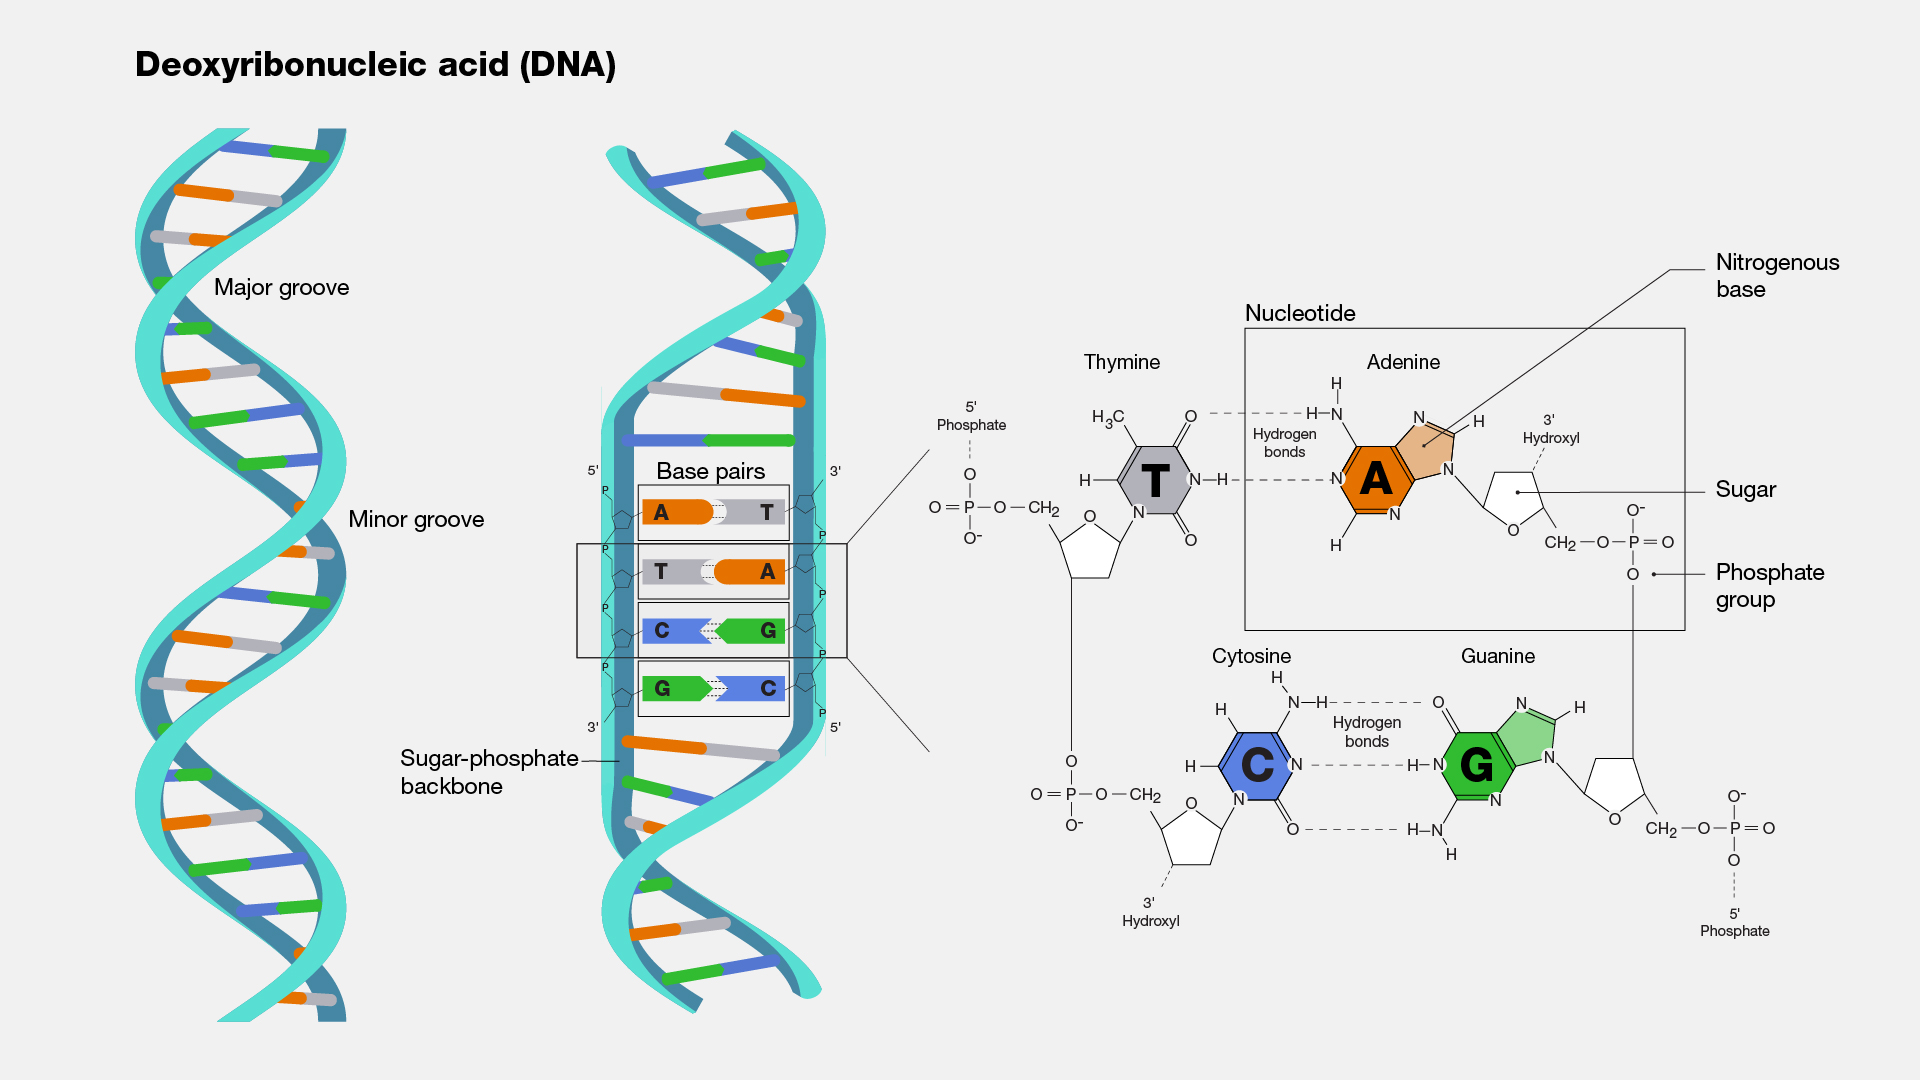
\includegraphics[width=.95\linewidth]{空间转录组学_CS_AI入门_讲义_配图/dna.jpg}
\caption{DNA 的结构与序列是两个观察视角。左侧为双螺旋，中间放大了碱基配对，右侧显示局部化学结构；A 与 T 配对，C 与 G 配对。入门时重点理解分子结构与字母序列的联系，无须记忆右侧化学细节。}\label{fig:handout-dna}
\par\smallskip{\footnotesize\color{muted}\raggedright 图片：\href{https://www.genome.gov/genetics-glossary/Deoxyribonucleic-Acid-DNA}{NHGRI}；许可：\href{https://www.genome.gov/about-nhgri/Policies-Guidance/Copyright}{Public domain}；原图等比缩放。\par}
\end{figure}
% END ADDED IMAGE dna

\subsection{基因是 DNA 上具有功能的一段信息}
基因不是整条 DNA 的另一个名字。一个基因对应 DNA 上的特定区段，可用于产生 RNA；许多基因最终与蛋白质的制造有关，还有一些基因产生的 RNA 本身就有功能。\cite{nhgri-glossary}

把 DNA 类比成一本很长的说明书，基因像其中一段有具体用途的内容。DNA 上也有参与调控等作用的区域，因此不能把全部 DNA 都当成一段段蛋白质制造说明。

\subsection{染色体和基因组怎么放进这张图}
DNA 会与蛋白质结合，组织成染色体。可以粗略把染色体理解成 DNA 的包装形式。基因组指一套遗传信息；它与“此刻表达了什么”是两个问题。\cite{nhgri-glossary}

\begin{center}
\rowcolors{2}{lightblue}{white}
\begin{tabularx}{\linewidth}{@{}l Y Y@{}}
\toprule
\rowcolor{tablehead}
概念 & 我们可以先这样记 & 不要混淆成 \\
\midrule
DNA & 保存遗传信息的分子 & 某一个基因 \\
基因 Gene & DNA 上具有功能的特定区段 & 整套遗传信息 \\
染色体 Chromosome & DNA 与蛋白质形成的组织结构 & 新的另一种信息分子 \\
基因组 Genome & 一套遗传信息 & 当前正在使用的信息集合 \\
\bottomrule
\end{tabularx}
\end{center}


% BEGIN ADDED IMAGE chromosome
\begin{figure}[!htbp]\centering
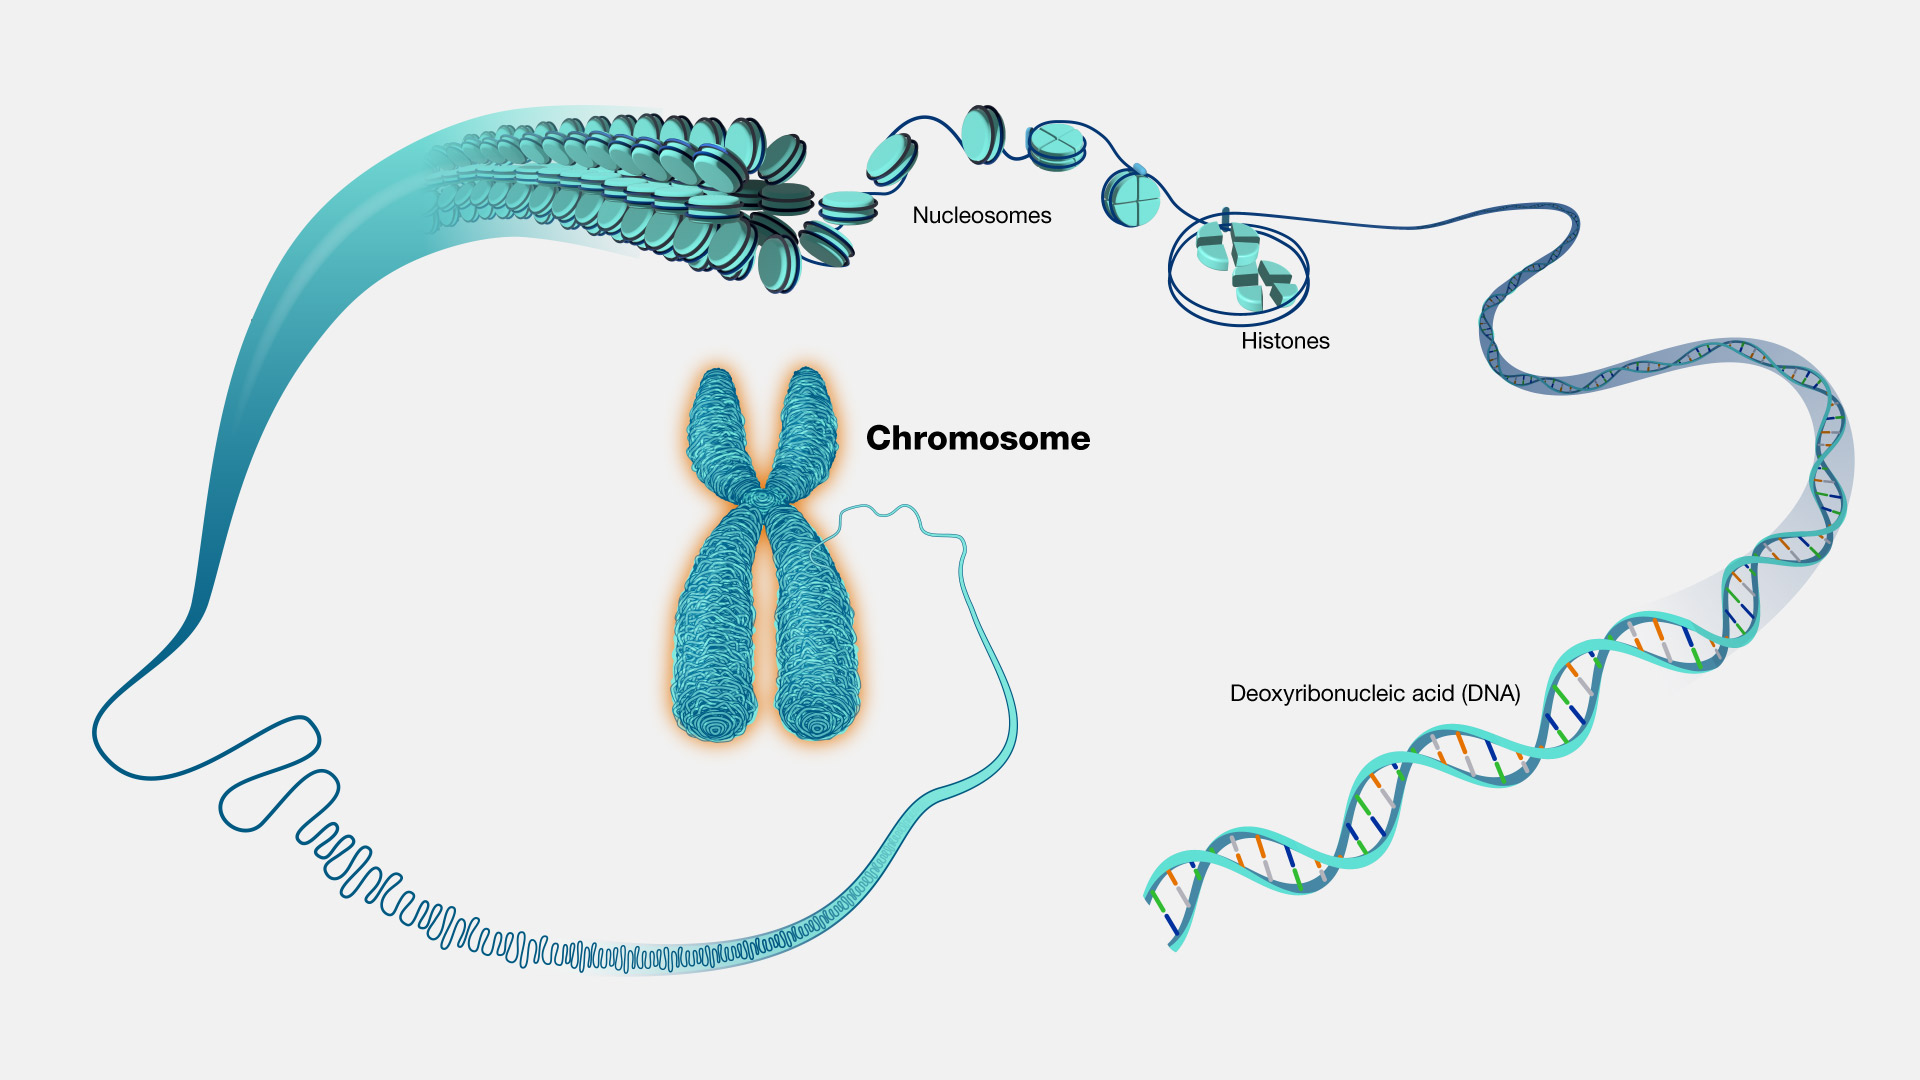
\includegraphics[width=.95\linewidth]{空间转录组学_CS_AI入门_讲义_配图/chromosome.jpg}
\caption{从 DNA 双螺旋到染色体的组织层次。可从右向左观察 DNA 如何与蛋白质结合并形成更高层次的包装；各部分不按统一比例绘制。图中的 X 形是特定阶段的结构示意，不表示染色体始终呈 X 形。}\label{fig:handout-chromosome}
\par\smallskip{\footnotesize\color{muted}\raggedright 图片：\href{https://www.genome.gov/genetics-glossary/Chromosome}{NHGRI}；许可：\href{https://www.genome.gov/about-nhgri/Policies-Guidance/Copyright}{Public domain}；原图等比缩放。\par}
\end{figure}
% END ADDED IMAGE chromosome

\subsection{为什么不同细胞可以拥有相似 DNA}
同一个人的多数有核体细胞，基因组大体相同。然而神经细胞和免疫细胞的工作明显不同。重要原因之一是：它们使用不同的基因，使用程度也不同。DNA 中“有这段信息”与细胞“现在正在使用这段信息”，需要分开。

\takeaway{基因是 DNA 的特定区段；基因存在，不代表它此刻被同样程度地使用。}

\chapterstart{RNA 是怎样产生的}
\subsection{细胞会按照 DNA 信息制造 RNA}
RNA 是另一类实际存在的分子。细胞按照 DNA 中的信息合成 RNA，这个过程叫\term{转录}{transcription}。DNA 并不是整条变成 RNA；细胞利用相应信息生成 RNA 分子，DNA 仍然存在。\cite{nhgri-transcription}

继续用说明书类比：DNA 是保存的信息，RNA 可以像为当前工作制作的副本。一段基因信息可以对应多个 RNA 分子，所以 RNA 的数量会随细胞状态变化。这里的“副本”强调信息关系，不表示 DNA 和 RNA 的化学组成完全相同。


% BEGIN ADDED IMAGE transcription
\begin{figure}[!htbp]\centering
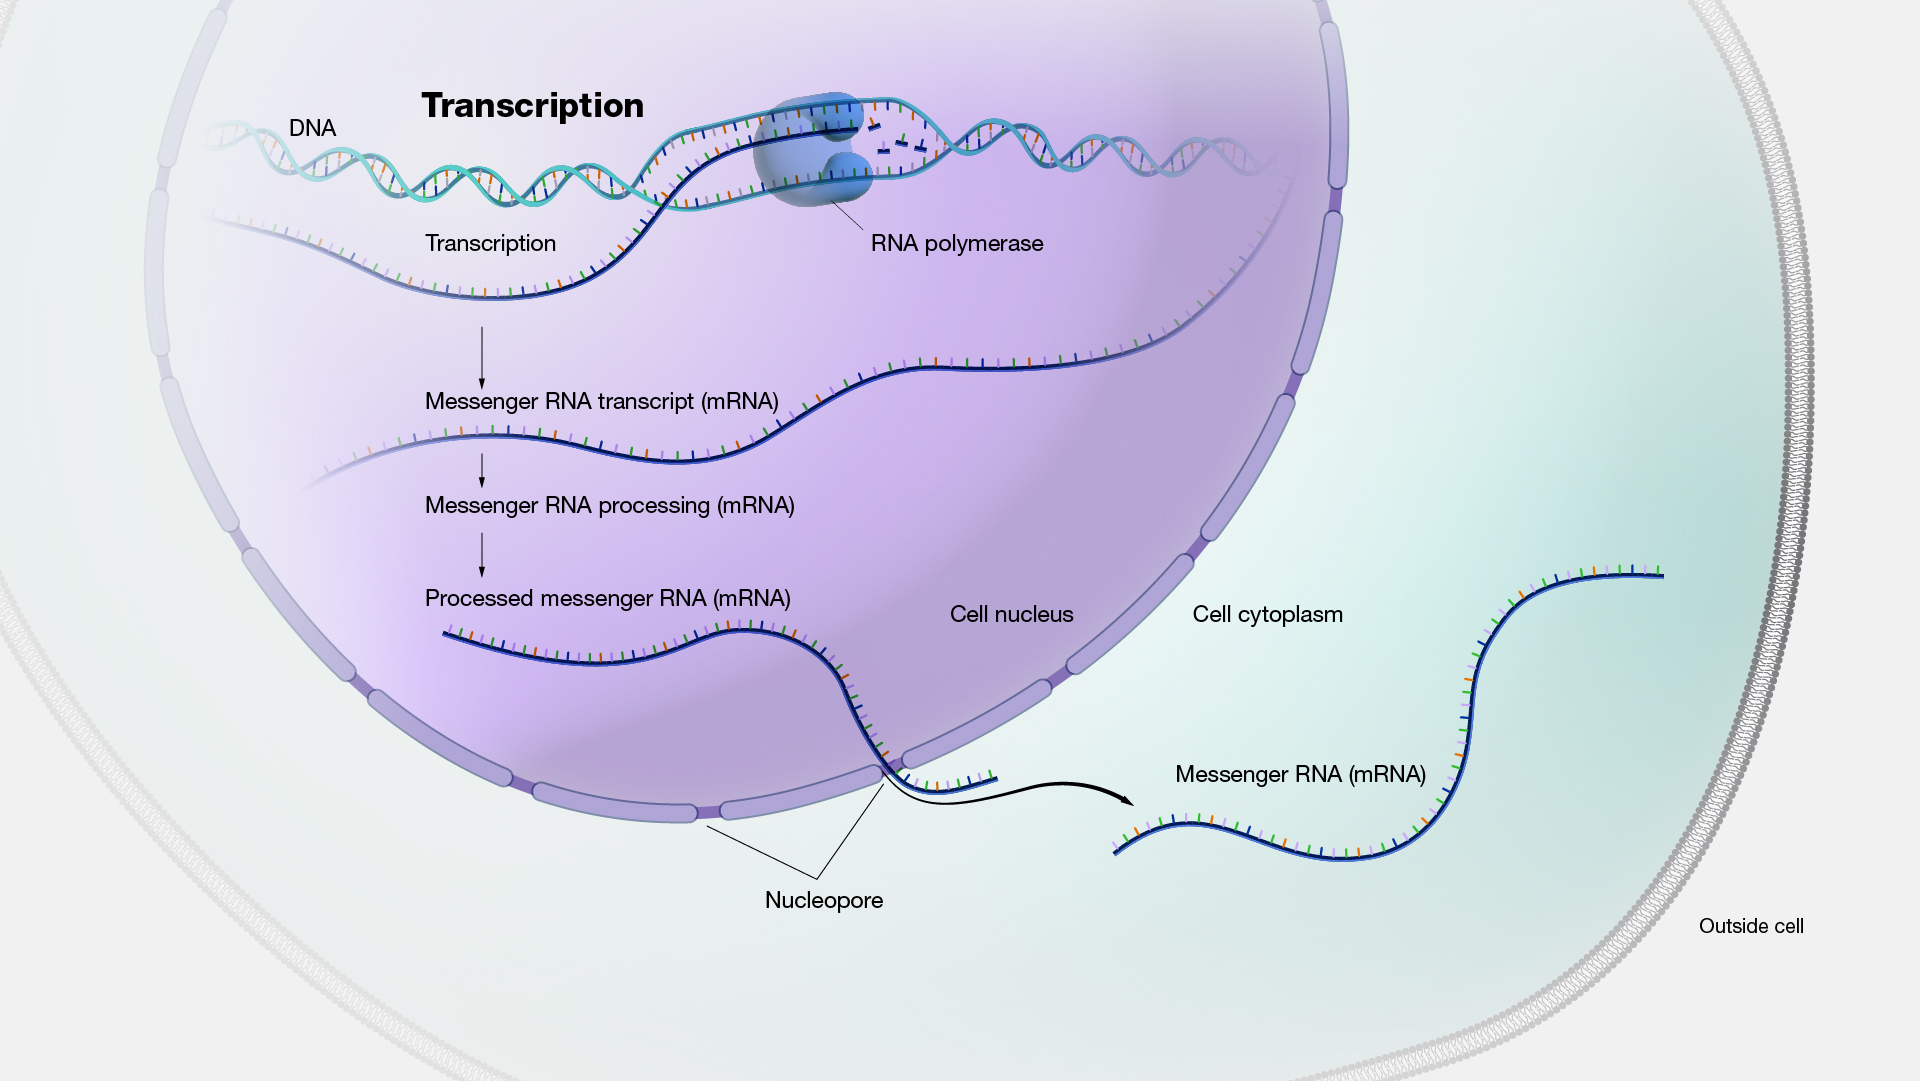
\includegraphics[width=.95\linewidth]{空间转录组学_CS_AI入门_讲义_配图/transcription.jpg}
\caption{真核细胞中的转录及 mRNA 加工示意。沿图自上而下观察：RNA 聚合酶根据 DNA 模板合成 RNA，mRNA 经加工后可经核孔离开细胞核。此图展示 mRNA 的典型路线，不表示所有 RNA 都会离核或进入翻译。}\label{fig:handout-transcription}
\par\smallskip{\footnotesize\color{muted}\raggedright 图片：\href{https://www.genome.gov/genetics-glossary/Transcription}{NHGRI}；许可：\href{https://www.genome.gov/about-nhgri/Policies-Guidance/Copyright}{Public domain}；原图等比缩放。\par}
\end{figure}
% END ADDED IMAGE transcription

\subsection{mRNA 是 RNA 中的一种}
mRNA 叫信使 RNA，它携带用于制造蛋白质的信息。RNA 还有其他类别，其中一些参与蛋白质制造的过程，另一些参与调控等功能。我们现在只需记住：\textbf{mRNA 是 RNA 的一个子类，不是所有 RNA 都是 mRNA。}\cite{nhgri-mrna}


% BEGIN ADDED IMAGE rna
\begin{figure}[!htbp]\centering
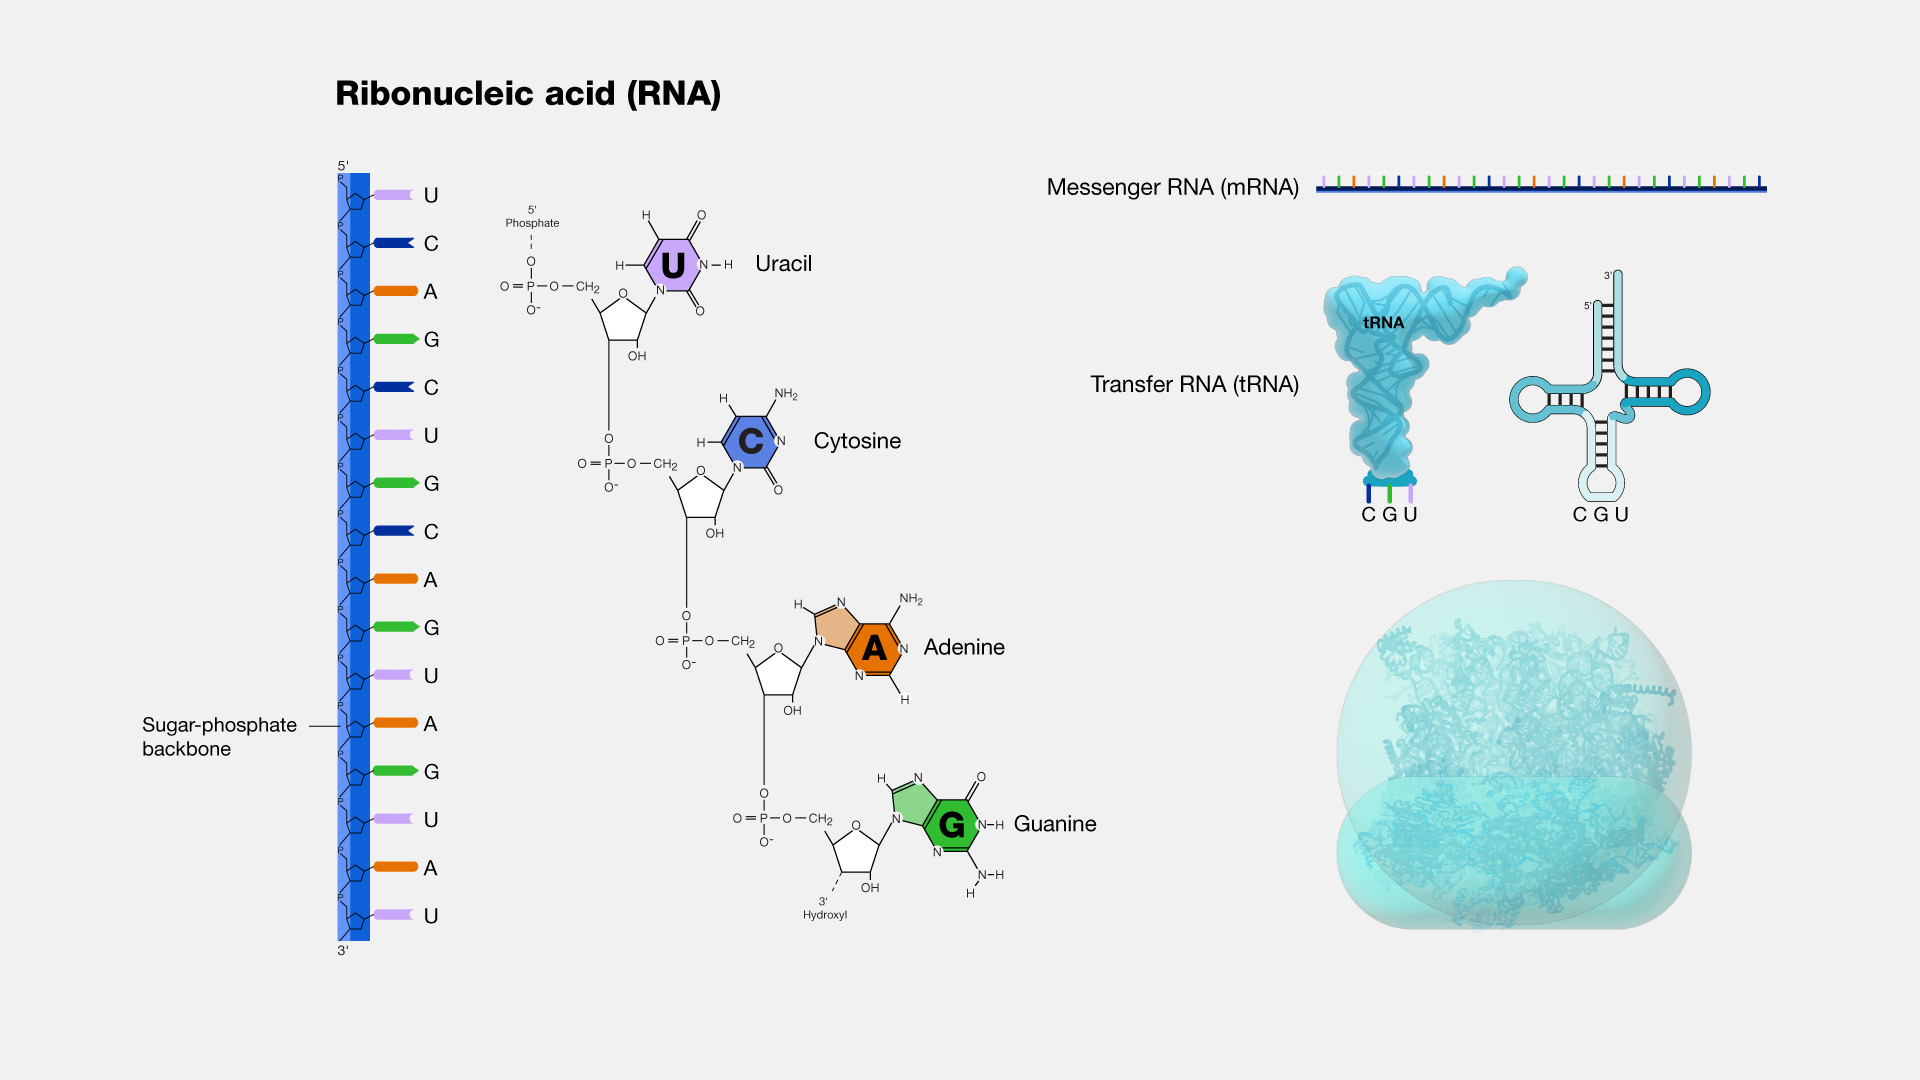
\includegraphics[width=.95\linewidth]{空间转录组学_CS_AI入门_讲义_配图/rna.jpg}
\caption{RNA 不只有 mRNA。右上方为信使 RNA（mRNA），其下展示转运 RNA（tRNA）和核糖体 RNA（rRNA）相关结构；后两者也参与蛋白质合成。RNA 可以形成复杂结构，不能把所有 RNA 都理解为等待翻译的一条直线。}\label{fig:handout-rna}
\par\smallskip{\footnotesize\color{muted}\raggedright 图片：\href{https://www.genome.gov/genetics-glossary/Ribonucleic-Acid-RNA}{NHGRI}；许可：\href{https://www.genome.gov/about-nhgri/Policies-Guidance/Copyright}{Public domain}；原图等比缩放。\par}
\end{figure}
% END ADDED IMAGE rna

\subsection{RNA 为什么能提供细胞状态的线索}
如果某类 RNA 在一个细胞中测得比较多，说明这个细胞在相应表达方面有一定信号。不同细胞会呈现不同的 RNA 组合；同一类细胞受到刺激后，组合也可能改变。通过这些组合，我们可以研究细胞的身份和状态。

但 RNA 水平不是“此刻产生速度”的直接读数。它同时受合成、降解及测量过程影响。我们测到的是实验所记录的 RNA 信号，再据此作解释。

\subsection{先把一个常见误解排除}
“DNA $\rightarrow$ RNA”表示信息通过转录被用于制造 RNA，不表示细胞把自己的 DNA 消耗掉。类似我们从文件生成多个工作副本，原文件仍然在，只是这个计算机类比忽略了许多真实分子过程。

\begin{center}
\rowcolors{2}{lightblue}{white}
\begin{tabularx}{\linewidth}{@{}Y Y@{}}
\toprule
\rowcolor{tablehead}
我们想知道什么 & 更相关的观察 \\
\midrule
细胞拥有哪些遗传信息 & DNA 或基因组信息 \\
细胞当时有哪些 RNA 信号 & RNA 或转录组信息 \\
细胞里有哪些功能性蛋白质 & 蛋白质相关测量 \\
\bottomrule
\end{tabularx}
\end{center}

回到我们的薄片：测 RNA 可以帮助识别免疫相关的表达特征，但并不是直接拍到了一个“免疫细胞标签”。我们后面还会解释怎样从信号推断身份。

\takeaway{转录根据 DNA 信息产生 RNA；测得的 RNA 水平为细胞身份和状态提供线索。}

\chapterstart{蛋白质是什么以及怎样产生}
\subsection{蛋白质由氨基酸链组成}
蛋白质是一类分子，通常由一条或多条氨基酸链构成。把氨基酸想成不同种类的小珠子：珠子按一定顺序连起来，链再折叠成一定形状。顺序影响结构，结构与功能密切相关。\cite{nhgri-protein}

单个蛋白质分子在分子尺度，肉眼看不见，普通光学显微镜通常也无法直接辨认其具体形状。但大量蛋白质构成的材料可以看见、摸到：头发富含角蛋白，肌肉含有参与收缩的蛋白质。蛋清也含有许多蛋白质，同时含大量水。


% BEGIN ADDED IMAGE protein
\begin{figure}[!htbp]\centering
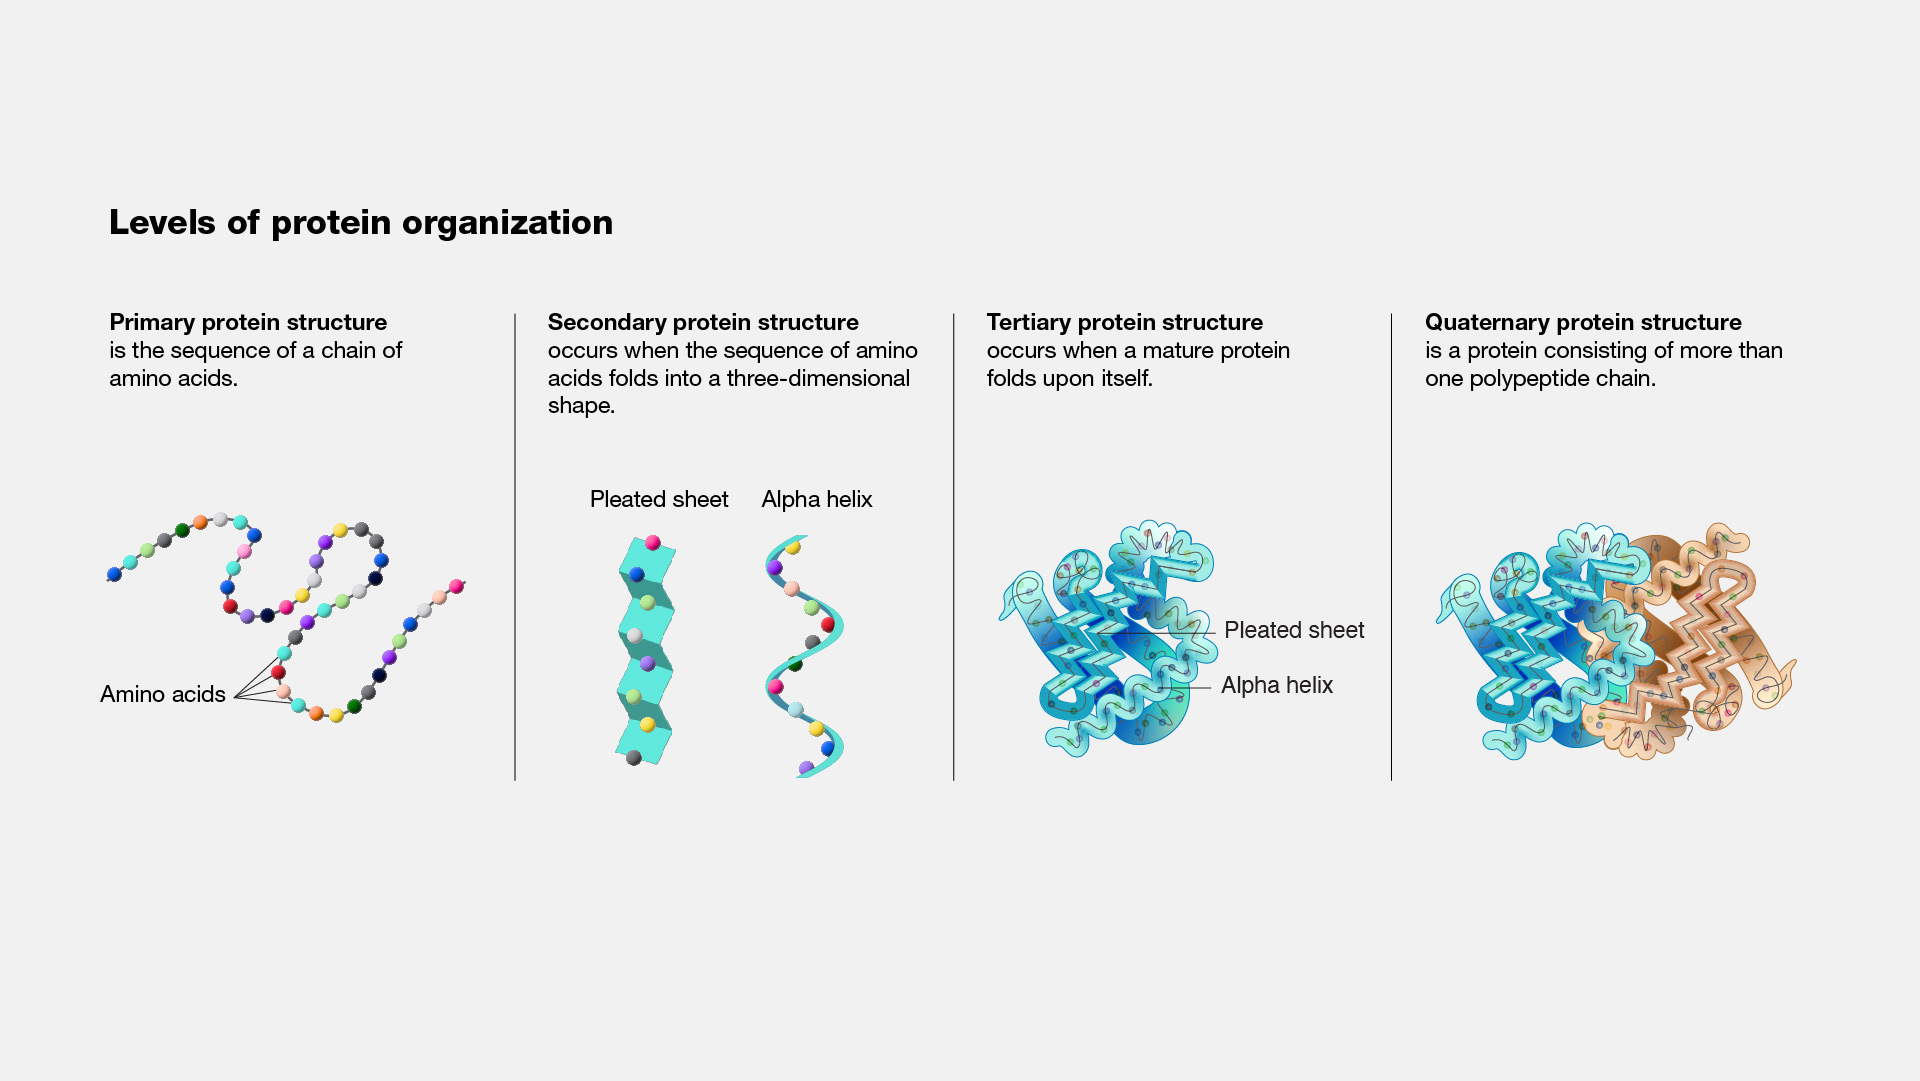
\includegraphics[width=.95\linewidth]{空间转录组学_CS_AI入门_讲义_配图/protein.jpg}
\caption{蛋白质的结构层次。从左到右依次为氨基酸序列、局部结构、整体折叠与多链组装；并非每种蛋白质都有多链组装这一层次。先理解“链具有顺序，也具有空间结构”，再将结构与功能联系起来。}\label{fig:handout-protein}
\par\smallskip{\footnotesize\color{muted}\raggedright 图片：\href{https://www.genome.gov/genetics-glossary/Protein}{NHGRI}；许可：\href{https://www.genome.gov/about-nhgri/Policies-Guidance/Copyright}{Public domain}；原图等比缩放。\par}
\end{figure}
% END ADDED IMAGE protein

\subsection{翻译把 mRNA 的信息用于制造蛋白质}
细胞中的核糖体等分子机器读取 mRNA 的信息，将氨基酸按相应顺序连接起来。这个过程叫\term{翻译}{translation}。这里的“翻译”是分子生物学术语，和自然语言翻译是不同任务。\cite{nhgri-translation}


% BEGIN ADDED IMAGE translation
\begin{figure}[!htbp]\centering
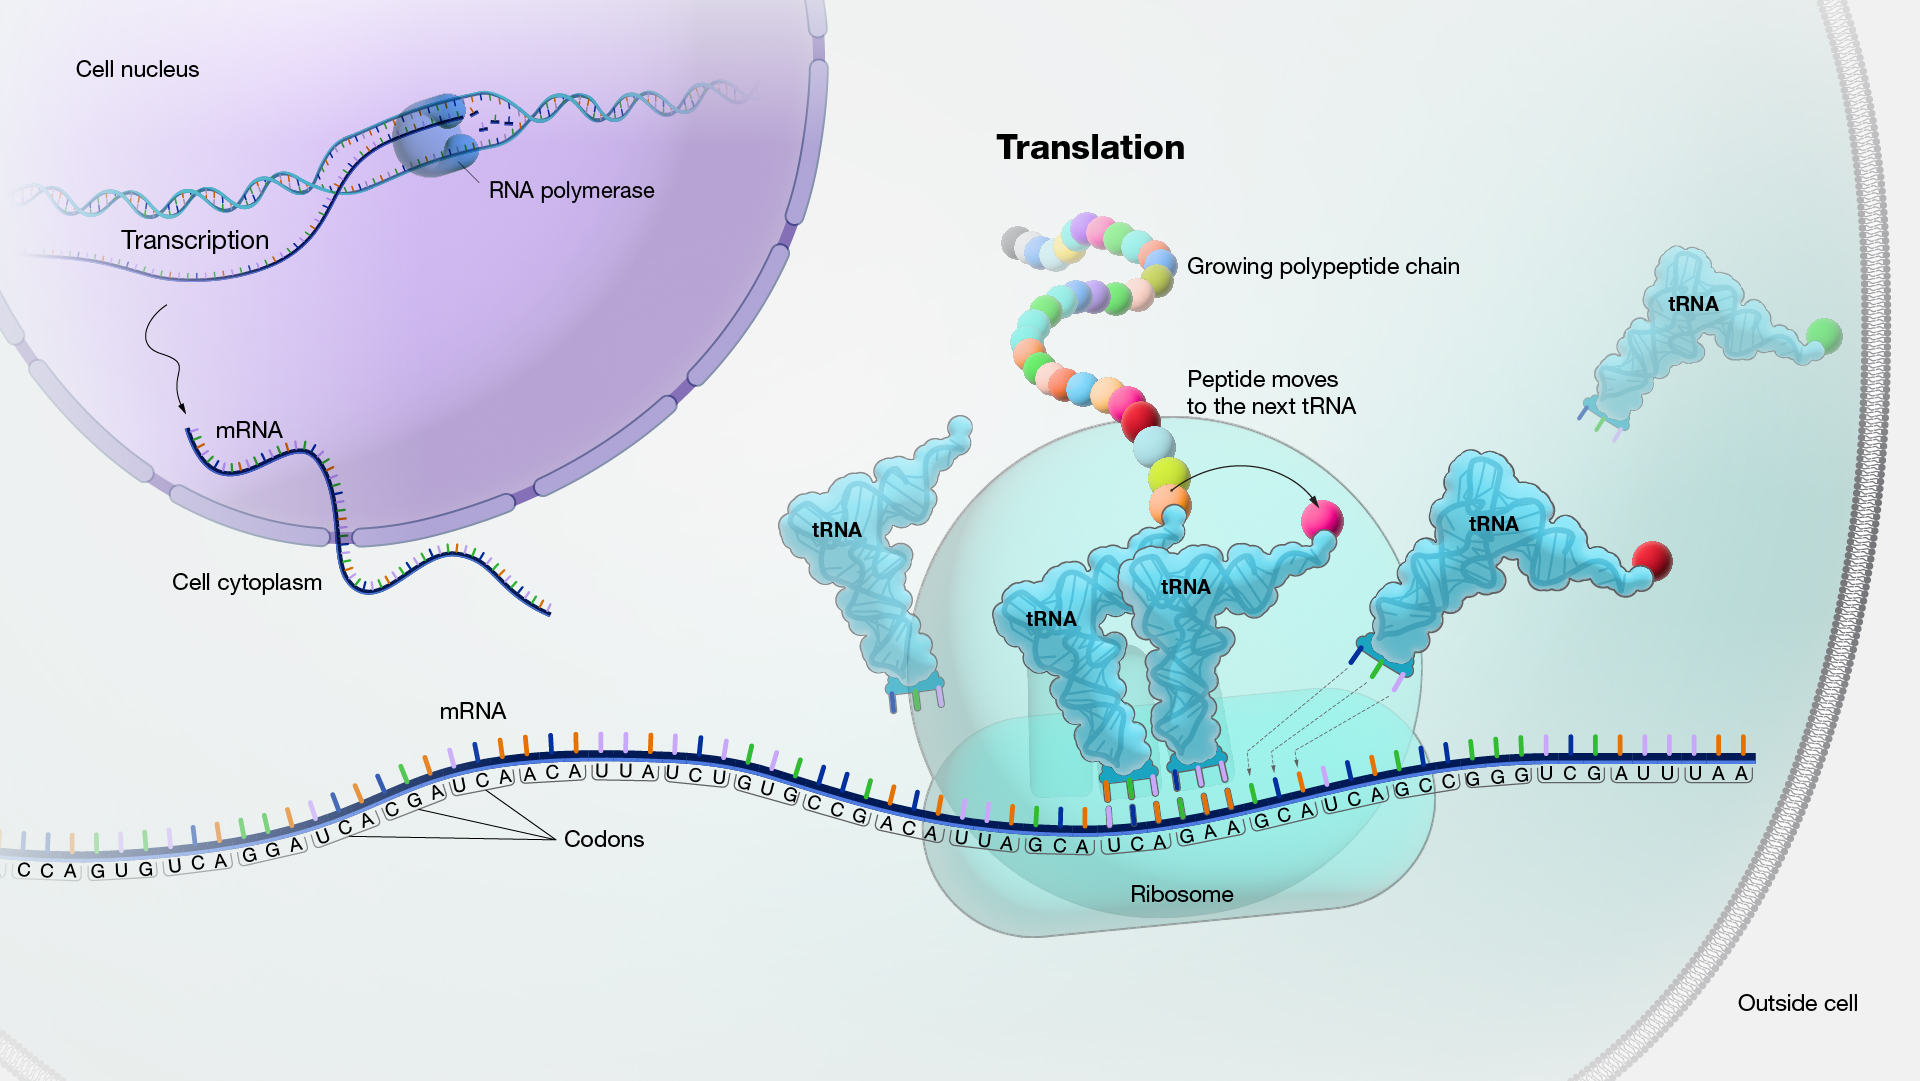
\includegraphics[width=.95\linewidth]{空间转录组学_CS_AI入门_讲义_配图/translation.jpg}
\caption{翻译过程示意。下方长链为 mRNA，蓝绿色结构为核糖体，正在延长的彩色小球串代表多肽链；tRNA 参与运送相应的氨基酸。RNA 提供编码信息，氨基酸构成多肽链，不能把翻译理解为 RNA 本身变成蛋白质。}\label{fig:handout-translation}
\par\smallskip{\footnotesize\color{muted}\raggedright 图片：\href{https://www.genome.gov/genetics-glossary/Translation}{NHGRI}；许可：\href{https://www.genome.gov/about-nhgri/Policies-Guidance/Copyright}{Public domain}；原图等比缩放。\par}
\end{figure}
% END ADDED IMAGE translation

\begin{figure}[htbp]
\centering
\begin{tikzpicture}[>=Stealth,font=\small]
  \draw[draw=accent,fill=lightblue,rounded corners] (0,0) rectangle (14,3.3);
  \node[anchor=west] at (0.3,3) {典型有核人体细胞的简化示意};
  \draw[draw=accent,fill=accent!12] (2.4,1.4) ellipse (1.7 and 1.1);
  \node at (2.4,1.95) {细胞核};
  \node at (2.4,1.15) {DNA 中的基因信息};
  \draw[->,thick,accent] (4.2,1.35) -- (6,1.35);
  \node at (5.1,1.85) {转录};
  \node at (7.1,1.35) {mRNA};
  \draw[->,thick,accent] (8.1,1.35) -- (10.3,1.35);
  \node at (9.2,1.85) {翻译};
  \node at (11.7,1.35) {蛋白质};
\end{tikzpicture}
\caption{信息关系示意，不按实际尺寸绘制。mRNA 在核内产生，参与蛋白质制造前通常需要加工并转运；图中省略这些步骤。部分 RNA 本身有功能，不进入翻译路线。}
\label{fig:dna-rna-protein}
\end{figure}

\subsection{为什么蛋白质重要}
许多具体工作由蛋白质承担：酶帮助化学反应进行，血红蛋白运输氧气，抗体参与防御，受体接收信号。受体可以先理解为细胞识别某些外来分子信号的组件。


% BEGIN ADDED IMAGE hemoglobin
\begin{figure}[!htbp]\centering
\begin{minipage}[c]{.42\linewidth}\centering 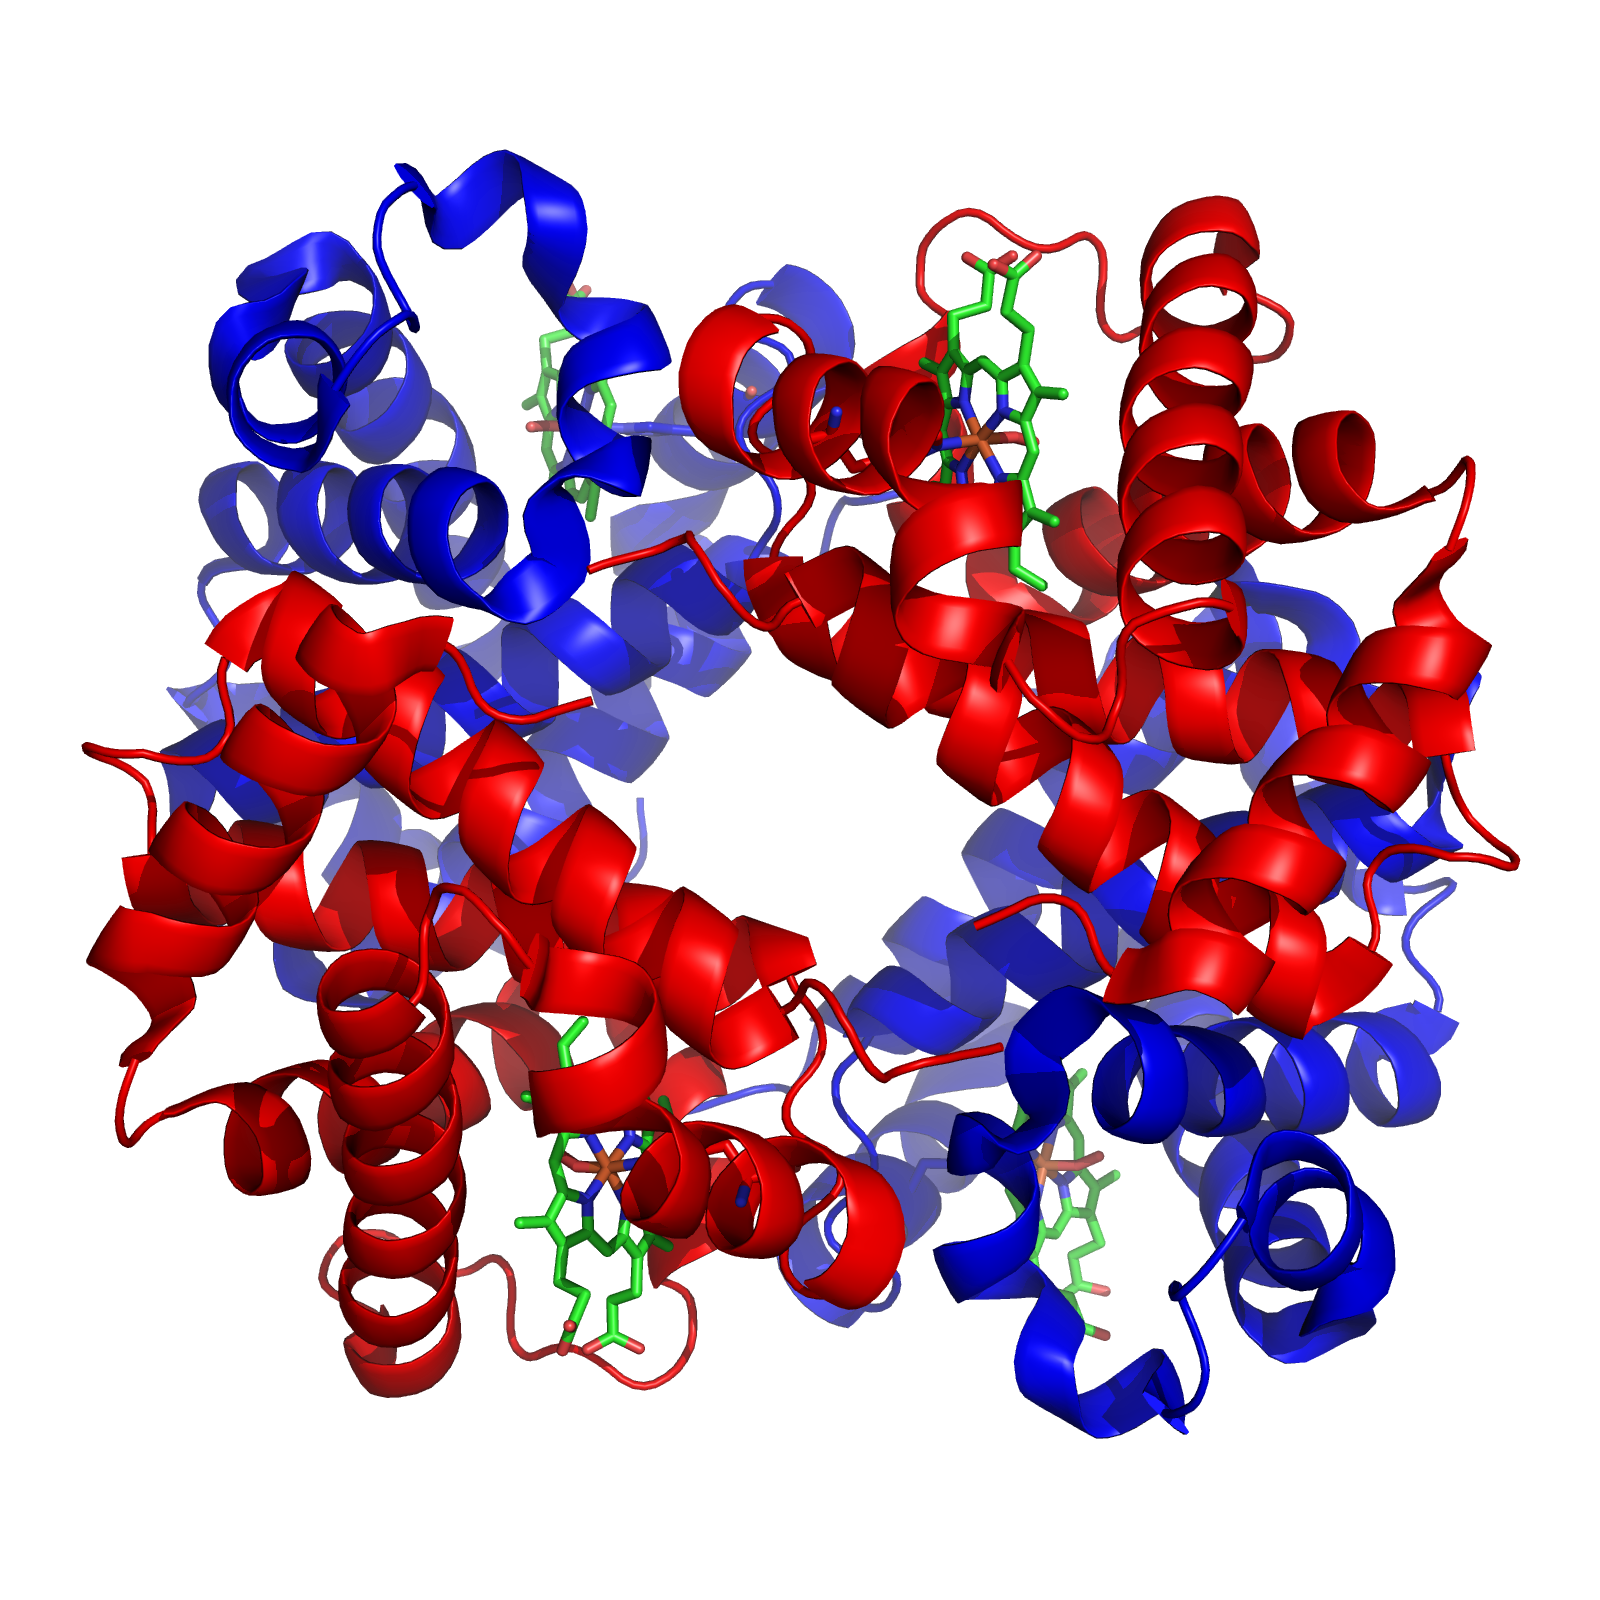
\includegraphics[width=.92\linewidth]{空间转录组学_CS_AI入门_讲义_配图/hemoglobin.png}\end{minipage}\hfill\begin{minipage}[c]{.53\linewidth}\small \textbf{把功能名词与具体结构联系起来。}血红蛋白是上文运输氧气的例子，这里可以看到蛋白质的空间结构。\par\medskip \textbf{再回到测量层次。}RNA 提供表达线索；若要判断蛋白质含量或功能是否发生变化，仍需相应证据。\end{minipage}
\caption{血红蛋白的三维结构模型，由 PDB 1GZX 的结构数据绘制，飘带帮助展示蛋白链的折叠。模型不是显微照片，绘图颜色也不是分子的真实颜色；它不能给出组织中的蛋白质含量。}\label{fig:handout-hemoglobin}
\par\smallskip{\footnotesize\color{muted}\raggedright 图片：\href{https://commons.wikimedia.org/wiki/File:1GZX_Haemoglobin.png}{Richard Wheeler (Zephyris)}；许可：\href{https://creativecommons.org/licenses/by-sa/3.0/}{CC BY-SA 3.0}；原图等比缩放。\par}
\end{figure}
% END ADDED IMAGE hemoglobin

\takeaway{DNA 保存信息；转录产生 RNA；其中的 mRNA 可被翻译成蛋白质；蛋白质承担许多实际功能。}

\chapterstart{基因表达是在说什么}
\subsection{表达表示基因信息被用于产生功能产物}
\term{基因表达}{gene expression}，是基因信息被用于产生 RNA 或蛋白质等功能产物的过程。研究 RNA 数据时，“某基因表达高”通常表示与这个基因相关的 RNA 信号测得较多。\cite{nhgri-expression}

例如，细胞甲和细胞乙都拥有某个基因，但在相同测量条件下，甲记录到更多对应 RNA。我们会说甲的这个基因表达较高。它并不表示甲拥有更多个基因，也不表示 DNA 序列变长了。

\subsection{为什么相似 DNA 能产生不同细胞}
细胞并不会同样程度地使用所有基因。不同的表达组合与细胞不同的结构、功能和状态有关。可以把它理解成：员工拥有相似的说明书，但当前执行的任务不同，生成的工作副本也不同。

\subsection{细胞类型和细胞状态要分开}
\term{细胞类型}{cell type}是较稳定的身份，例如免疫细胞中的 T 细胞；\term{细胞状态}{cell state}是当下的活动情况，例如应对刺激或正在增殖。增殖就是细胞分裂、数量增加相关的过程。

同一种类型可以有不同状态，不同类型也可能共享一种状态。例如，多个类型都可能处于增殖状态。算法把细胞分成两组后，需要判断分组反映的是身份、状态，还是实验差异。

\subsection{标志基因怎样帮助识别细胞}
某些基因的表达常为识别细胞身份或状态提供线索，我们称它们为\term{标志基因}{marker gene}。科研人员通常结合多个标志、已有研究和组织背景判断，而不是看到一个基因较高就给出确定标签。

\subsection{RNA 多为什么不一定等于蛋白质多}
从 RNA 到蛋白质，中间还有翻译效率和蛋白质降解等过程。测 RNA 是一个观测层次，测蛋白质是另一个观测层次。RNA 数据可以提出功能相关假设，但不自动证明蛋白质数量或功能强度发生了相同变化。

\checkpoint{基因是信息区段，表达是信息被使用；细胞类型是身份，细胞状态是当下情况。空间转录组主要提供 RNA 层面的表达线索。请试着解释：两个细胞拥有相似的 DNA，为什么仍可能表现出不同的功能？}

\partdivider{测量原理与空间信息}{第 6--9 章：从 RNA 集合到带位置的实验读数}{%
  理解转录组测量的范围和局限，比较混合组织、单细胞与空间测量。弄清一个测量单位代表什么，以及条形码、UMI 和成像怎样把 RNA 信号与位置关联起来。}

\chapterstart{转录组是很多 RNA 的整体情况}
\subsection{先理解为什么要加一个“组”字}
只测一个基因，可以看到一个信号；同时测很多基因，才能看到整体的表达组合。\term{转录组}{transcriptome}指一个细胞或组织在特定条件下的 RNA 集合。\cite{nhgri-transcriptome}

我们可以把它理解为一份“当时的 RNA 情况表”。它与基因组不同：基因组主要描述保存的遗传信息，转录组描述当时存在的 RNA。细胞的环境或状态改变时，转录组也可能变化。

\subsection{一个基因和一个 RNA 分子不是一一对应}
一个基因可以产生很多 RNA 分子。一个基因也可能产生不同的\term{转录本}{transcript}。这里的转录本可以先理解为 RNA 产物；谈“转录本种类”时，也可能在区分同一基因产生的不同版本。

在常见入门分析中，研究人员会把与同一基因有关的信号汇总到基因层面。因此表达表的一列常是一个基因，数值反映该基因相关信号，而不是说“每个基因只有一个 RNA”。

\subsection{测转录组不等于测到了所有 RNA}
真实实验存在捕获效率、测序投入和技术覆盖范围的限制。有些方案关注较广的转录组，有些只检测预先选定的一组基因。这组目标叫 \term{panel}{基因面板}，可以先理解为实验事先决定的“测量名单”。

因此，数据里没看到某个 RNA 信号，不能直接说细胞完全没有它。尤其某个基因根本不在测量名单中时，它属于没有观测，不能当成确定的零表达。

对 CS / AI 读者来说，这里要区分两种情况：“测了这个特征但读数为零”，以及“实验根本没有测这个特征”。即使文件里都能用零填充，它们的含义也不相同。

\subsection{RNA 测量怎样帮助研究组织}
假设免疫相关的一组基因在某些区域更明显，研究人员就有理由进一步检查这些区域是否含有免疫细胞。表达模式提供线索，已有参考和额外验证帮助判断线索是否可靠。

我们还没有加入空间。下一步先看看：如果同样测 RNA，但把细胞合在一起或分开测，会得到哪些不同信息。

\takeaway{转录组是一组 RNA 的整体情况；表达数据是对它的不完整测量。}

\chapterstart{混在一起测和分开测有什么区别}
\subsection{第一种方式是测一份混合组织}
如果把一块组织中的 RNA 汇总来测，我们得到整份样本的总体表达情况。这类方法常叫 \textbf{bulk RNA-seq}，bulk（批量） 可以先理解为“混合在一起”。RNA-seq 指通过测序来研究 RNA。\cite{nhgri-rnaseq}

它像把公司的工作记录全部汇总：我们能知道整个公司用了哪些任务信息，但很难区分每条记录来自哪个员工。某个信号变多，可能是相关员工变多，也可能是每个人的活动更强。

\subsection{第二种方式是尽量分别测每个细胞}
\textbf{单细胞 RNA 测序}，简称 \textbf{scRNA-seq}（sc：single-cell），尽量把不同细胞的 RNA 信号分开记录。于是可以比较不同细胞，发现它们有哪些身份和状态差异。常见实验需要将细胞从组织中\textbf{解离}，也就是从原来的结构里分离出来。

这像分别保存每个员工的工作记录，但通常丢失了他们原来的座位。并非所有细胞都能成功进入数据，一次记录也可能混入多个细胞，所以仍然需要质量检查。

\begin{center}
\rowcolors{2}{lightblue}{white}
\begin{tabularx}{\linewidth}{@{}l Y Y@{}}
\toprule
\rowcolor{tablehead}
研究方式 & 得到什么 & 暂时看不到什么 \\
\midrule
混合组织测量 & 整份组织的总体表达 & 每种细胞各自贡献多少 \\
单细胞测量 & 分别记录细胞间的表达差异 & 常规解离后细胞原来的组织位置 \\
\bottomrule
\end{tabularx}
\end{center}

\subsection{单细胞核又是什么}
一些实验分离并测量细胞核，称为\textbf{单细胞核 RNA 测序}，简称 \textbf{snRNA-seq}。细胞核是细胞的一部分，因此核内 RNA 与整个细胞 RNA 的构成不完全相同。现在只需知道：single-cell 和 single-nucleus 不是完全相同的测量对象。

\subsection{我们的研究问题还缺什么}
对肿瘤薄片，即使知道存在多少种免疫细胞，我们仍想知道它们在内部还是边缘、与哪些细胞相邻。仅有总体表达或失去原位坐标的单细胞表，都不能直接完整回答这个布局问题。

\takeaway{bulk 看总体，单细胞看个体差异；想研究组织布局，还要保留位置。}

\chapterstart{空间转录组把表达放回组织地图}
\subsection{空间转录组同时关联表达和位置}
\term{空间转录组学}{spatial transcriptomics}，是在保留空间位置关联的条件下测量组织中的 RNA 表达。它让我们研究“哪些表达信号出现在哪里”，以及这些位置之间的关系。\cite{stahl2016}

把公司类比补完整：我们有员工的工作记录，也保留座位图。研究对象由一份没有布局的信息表，变成了一张具有表达信息的组织地图。


% BEGIN ADDED IMAGE spatial
\begin{figure}[!htbp]\centering
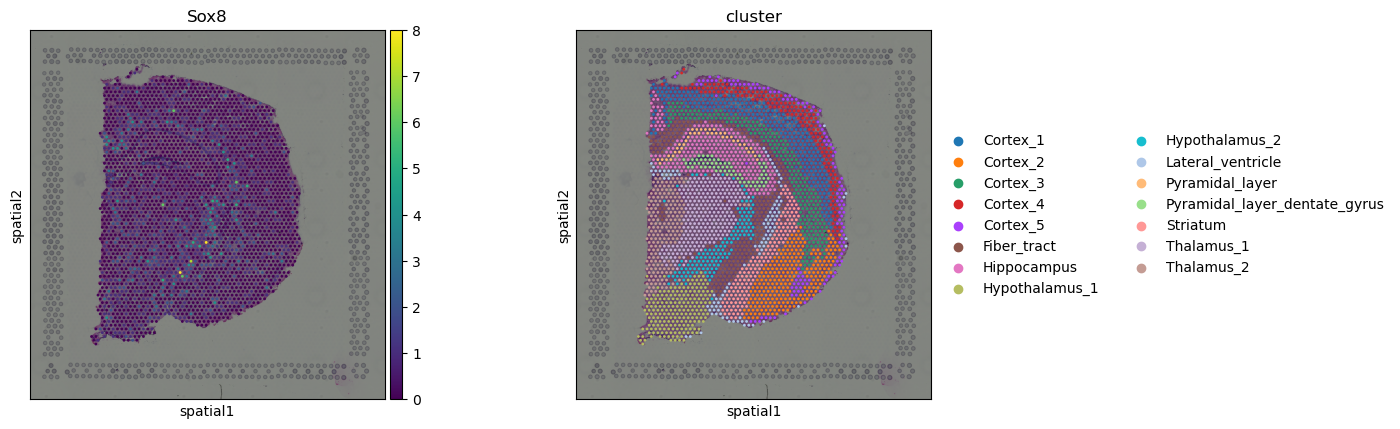
\includegraphics[width=.95\linewidth]{空间转录组学_CS_AI入门_讲义_配图/spatial.png}
\caption{空间数据的真实可视化示例，来自 Squidpy 官方 Visium 教程。左图用连续颜色表示 Sox8 表达信号（表达量），右图用离散颜色显示分群及注释标签（属于哪个空间），两图使用同一组织的空间位置。圆点代表测量位置，不自动等于单个细胞；注释标签包含分析与解释，并非实验直接读出的身份。}\label{fig:handout-spatial}
\par\smallskip{\footnotesize\color{muted}\raggedright 图片：\href{https://squidpy.readthedocs.io/en/latest/notebooks/examples/plotting/plot_scatter.html}{Squidpy / Theis Lab / scverse}；许可：\href{https://github.com/scverse/squidpy/blob/main/LICENSE}{BSD 3-Clause}；原图等比缩放。\par}
\end{figure}
% END ADDED IMAGE spatial

\subsection{为什么位置有生物学意义}
组织的功能依赖细胞的排列与局部环境。免疫细胞集中在肿瘤边缘或出现在内部，是两个不同的观察；脑组织不同结构层的表达模式，也可能不同。位置帮助研究人员提出更具体的问题，但布局本身不直接证明某个功能或因果关系。

\subsection{空间不意味着每一行都是一个细胞}
不同技术的测量单位不同。有些数据对应分割得到的细胞，有些对应一个捕获区域。捕获区域常叫 \textbf{spot}，我们可以先把它想成组织上的一个小圆圈或小区域，里面可能有多个细胞。

较细的网格也可能被合并成 \textbf{bin}，即一个用于分析的网格区域。无论它多小，网格边界都不自动等于细胞边界。一份数据到底是在测细胞、spot 还是 bin，要看实验和后续处理。

\begin{center}
\rowcolors{2}{lightblue}{white}
\begin{tabularx}{\linewidth}{@{}p{2.8cm} Y Y@{}}
\toprule
\rowcolor{tablehead}
一行对应的对象 & 我们能直接说什么 & 我们还不能直接说什么 \\
\midrule
分割得到的细胞 & 该细胞区域记录到的 RNA & 分割及分子归属完全正确 \\
多细胞 spot & 该区域的混合 RNA 信号 & 每个细胞分别表达多少 \\
合并网格 bin & 该网格区域的 RNA 信号 & 这个网格就是一个完整细胞 \\
\bottomrule
\end{tabularx}
\end{center}

常见实验测量一张二维组织切片。二维坐标保留切片中的位置，不能直接代表完整器官的三维结构。研究三维组织时，通常还需要多个切片或其他信息。

\takeaway{转录组提供 RNA 表达信息，空间保留这些信息在组织中的位置；分析前先确认一个观测位置究竟代表什么。}

\chapterstart{实验怎样知道哪些 RNA 来自哪里}
\subsection{先看一种典型的测序路线}
下面以捕获 RNA 的空间条形码方案为例。研究人员准备一张载体，上面不同捕获位置带有不同的条形码序列。\term{条形码}{barcode}可以先理解成位置标签；实验知道每个标签对应哪个位置。

将组织薄片放在载体上，捕获到的 RNA 经实验处理获得相关标签，再进行测序。测序仪读到的序列片段叫 \textbf{read}。计算流程识别标签以及目标基因，便能把分子信号关联回位置。2016 年的经典空间转录组工作采用了这一类思路。\cite{stahl2016}

\subsection{一份读数要回答两个问题}
\begin{center}
\rowcolors{2}{lightblue}{white}
\begin{tabularx}{\linewidth}{@{}l Y Y@{}}
\toprule
\rowcolor{tablehead}
问题 & 帮助回答的信息 & 通俗理解 \\
\midrule
来自哪里 & 空间条形码和对应坐标 & 包裹上的地址标签 \\
属于哪个目标 & RNA 对应的序列或探针信息 & 包裹内容的识别线索 \\
\bottomrule
\end{tabularx}
\end{center}

实验常将 RNA 的信息转换到适合建库和测序的 DNA 产物上，再测序；这不改变我们研究的对象是 RNA 表达。这里省略实验化学细节，但要避免把“测序仪读到 DNA 产物”误解为“正在研究基因组突变”。\cite{nhgri-rnaseq}

这里的\textbf{建库}，可以先理解为把分子处理成测序仪可以读取的一组材料；它不是建立计算机数据库。

\subsection{为什么多个 reads 不一定等于多个 RNA}
建库中的扩增可能让一个原始分子产生多个副本，因此多个 reads 可能来源（比如经过PCR扩增）。部分方案加入 \term{UMI}{unique molecular identifier，独特分子标识符}，帮助识别重复来源。可以把空间条形码理解为“位置标签”，把 UMI 理解为“分子去重线索”。\cite{tenx-glossary}

例如，在同一位置、同一基因下，若若干 reads 具有相同的 UMI，流程可能把它们合并为一个分子来源的计数。真实去重还涉及序列错误等问题，因此这个例子只说明“reads 数量”和“去重后的分子计数”为何可能不同。

\subsection{另一条路线是直接在组织里成像}
成像型方法使用探针等分子工具识别目标，并通过显微成像及多轮识别等过程定位 RNA。\textbf{探针}可以先理解为实验中识别特定目标的工具。它可能输出“某种 RNA 在坐标哪里”的分子表，再聚合到细胞或区域。\cite{tenx-spatial}

\takeaway{先理解两条思路：通过标签保留位置，或通过成像定位分子。不同方案能检测什么、测得多细、测得多完整，会影响后续计算问题。现在不用背平台名。}

\partdivider{计算分析与科研实践}{第 10--15 章：从表达矩阵到可信科学结论}{%
  把实验读数转成矩阵、坐标与图像，理解常见分析步骤及算法任务。沿着肿瘤切片的例子，分清测量、推断、比较和验证，学习判断模型输出能支持怎样的结论。}


\begingroup
\setlength{\parskip}{0pt}
\chapterstart{从 RNA 读数到基因表达矩阵}

上一章，我们了解了实验如何识别 RNA 来自哪个位置、属于哪个基因。接下来需要解决一个问题：\textbf{如何把这些 RNA 信号整理成计算机可以分析的数据？}

答案就是将它们整理成一张矩阵。在空间转录组研究中，这张矩阵叫作\term{基因表达矩阵}{gene expression matrix}。

\subsection{把 RNA 信号整理成一张表}

假设我们有一张组织切片，其中包含四个捕获位置（spot），分别记为 P1、P2、P3 和 P4。

实验完成后，我们统计每个位置检测到了多少与不同基因对应的 RNA 信号，就可以得到下面这张表：

\begin{center}
\rowcolors{2}{lightblue}{white}
\begin{tabular}{@{}l r r r@{}}
\toprule
\rowcolor{tablehead}
位置 & 基因 A & 基因 B & 基因 C \\
\midrule
P1 & 30 & 2 & 5 \\
P2 & 27 & 3 & 8 \\
P3 & 3 & 28 & 4 \\
P4 & 16 & 17 & 6 \\
\bottomrule
\end{tabular}
\end{center}

例如，P1 中基因 A 的计数为 30，基因 B 为 2，基因 C 为 5。这说明在 P1 位置，实验检测到的基因 A 表达信号比另外两个基因更丰富。

这里的数字只是教学示例。真实数据中的基因通常使用具体名称或 ID，例如 EPCAM、PTPRC 等。不同基因的表达可以为判断细胞类型提供线索，但通常需要结合多个标志基因，而不能只依赖某一个基因。

\subsection{从 CS 的角度理解这张矩阵}

对于 CS 学生来说，基因表达矩阵其实就是一张熟悉的\textbf{特征矩阵（Feature Matrix）}。

我们可以这样理解：

\begin{itemize}
  \item \textbf{每一行是一个样本}：在空间转录组中，通常对应一个 spot；在单细胞数据中，则可能对应一个 cell。
  \item \textbf{每一列是一个特征}：这里的特征就是基因。
  \item \textbf{每个数值是表达计数}：表示实验在该位置记录到了多少与对应基因相关的 RNA 分子信号。
\end{itemize}

例如，P1 可以表示为一个三维特征向量：

\[
  X_1=[30,2,5]
\]

P2、P3 和 P4 也各自对应一个向量。把这些向量按行排列起来，就得到了完整的表达矩阵：

\[
  X=
  \begin{bmatrix}
  30 & 2 & 5\\
  27 & 3 & 8\\
  3 & 28 & 4\\
  16 & 17 & 6
  \end{bmatrix}
\]

在实际研究中，基因数量可能达到几千甚至几万个，因此每个 spot 对应的就是一个高维特征向量。

数学上，原始计数矩阵通常表示为：

\[
  X\in\mathbb{N}_0^{N\times G}
\]

其中，$N$ 表示观测单位（spot 或 cell）的数量，$G$ 表示基因数量，$\mathbb{N}_0$ 表示包含零的非负整数集合。

矩阵中的元素 $X_{ig}$ 表示第 $i$ 个观测单位中，第 $g$ 个基因的记录计数。

需要注意，\textbf{表达计数不是基因的数量。}例如，P1 中基因 A 的计数为 30，并不是说 P1 有 30 个基因 A，而是实验记录到了与基因 A 对应的 RNA 表达信号。由于捕获效率、测序误差等因素，这个数字也不一定等于真实存在的 RNA 分子数量。

另外，原始计数矩阵通常还需要经过归一化、对数变换等预处理。处理后的数值可能是小数，某些标准化表示中甚至会出现负数，因此一般可以写作：

\[
  X\in\mathbb{R}^{N\times G}
\]

所以，拿到一份表达矩阵时，首先要确认它保存的是原始计数，还是已经处理过的表达值。本文后续统一采用“观测单位 $\times$ 基因”的矩阵结构。


\subsection{如何从矩阵中观察表达模式}

有了基因表达矩阵，我们就可以开始比较不同位置的基因表达特征。

回到最开始的例子：

\begin{itemize}
  \item \textbf{P1 和 P2}：基因 A 的表达计数较高，基因 B 较低，因此两者的表达模式比较相似。
  \item \textbf{P3}：基因 B 的表达计数较高，和 P1、P2 呈现出不同的表达模式。
  \item \textbf{P4}：基因 A 和 B 都有较高的表达计数，说明这个位置同时检测到了两种表达信号。
\end{itemize}

假设基因 A 是上皮细胞的标志基因，基因 B 是免疫细胞的标志基因，那么我们可能会猜测：P1、P2 更接近上皮细胞相关区域，而 P3 可能具有免疫细胞相关特征。

但是，P4 同时表达 A 和 B，是否说明一个细胞同时具有上皮细胞和免疫细胞两种身份？

\textbf{不能直接这样判断。}

因为一个 spot 不一定只包含一个细胞。例如，P4 可能同时覆盖了上皮细胞和免疫细胞，测量结果实际上混合了多个细胞的 RNA 信号。

即使 P4 对应单个细胞，也需要考虑真实的基因共表达、背景污染或细胞分割误差等可能性。

因此，\textbf{基因表达矩阵能够帮助我们发现表达模式，但不能仅凭几个基因的表达值，就直接确定细胞类型。}

\subsection{矩阵里的零意味着什么}

最后还有一个很容易产生误解的地方：如果某个基因的表达计数为 0，是不是说明这个位置完全没有表达该基因？

答案是不一定。

在空间转录组实验中，RNA 的捕获和测序并不是百分之百准确的。即使某个基因确实发生了表达，也可能因为表达量太低、捕获效率有限或测序深度不足，最终没有被记录下来。此，表达矩阵中的零，首先表示\textbf{实验没有检测到对应的表达信号}，而不一定表示该基因在生物学上完全没有表达。

这也是为什么在后续的数据预处理和建模中，我们需要谨慎处理零值：不能把所有零都当作真实的无表达，也不能认为所有零都是需要补齐的缺失数据。




\clearpage
\endgroup
\chapterstart{坐标、图像和文件怎样与矩阵对应}

上一章，我们已经把 RNA 测序得到的信号整理成了基因表达矩阵。
矩阵的每一行对应一个 spot（空间捕获位置），每一列对应一个基因，
其中的数值表示该位置检测到的基因表达信号。

但这里还有一个问题：\textbf{我们知道每个 spot 表达了哪些基因，
却还不知道这些 spot 在真实组织中分别位于哪里。}

因此，空间转录组数据通常不只有基因表达矩阵，
还需要保存空间坐标，有时还会包含组织图像。
这几类数据结合起来，才能帮助我们理解基因表达与组织空间结构之间的关系。

\subsection{表达矩阵之外还要有坐标}

继续使用上一章的四个位置 P1、P2、P3 和 P4。

假设我们已经得到它们的基因表达矩阵，
现在再为每个位置记录一个二维坐标：

\[
  P1=(0,0),\quad P2=(1,0),\quad
  P3=(0,1),\quad P4=(1,1).
\]

这样，我们就有了两张相互关联的表：

\begin{itemize}
  \item \textbf{基因表达表}：记录每个 spot 中各个基因的表达情况。
  \item \textbf{空间坐标表}：记录每个 spot 在组织中的位置。
\end{itemize}

例如，基因表达表告诉我们 P1 中基因 A 的计数为 30；
空间坐标表则告诉我们 P1 位于 $(0,0)$。
将两者结合，就能知道某个基因在组织的什么位置表达较高。

从 CS 的角度看，这类似于数据库中的两张表：
一张保存特征，另一张保存坐标，通过共同的 spot ID 进行关联。

用数学语言表示，基因表达矩阵为

\[
X\in\mathbb{R}^{N\times G},
\]

其中 $N$ 是观测位置数，$G$ 是基因数。

对应的空间坐标矩阵为

\[
S\in\mathbb{R}^{N\times 2},
\]

其中每一行保存一个位置的 $(x,y)$ 坐标。

\textbf{这里最重要的是：$X$ 和 $S$ 的同一行，
必须对应同一个 spot。}

例如，如果 $X$ 的第一行是 P1 的基因表达，
那么 $S$ 的第一行也必须是 P1 的坐标。
实际处理数据时，应根据 spot ID 检查对应关系，
不能仅凭两个矩阵的行数相同，就认为它们已经正确对齐。

\begin{figure}[htbp]
\centering
\begin{tikzpicture}[font=\small]
  \node at (2.2,3.45) {表达计数};
  \foreach \x/\lab in {0.8/A,1.7/B,2.6/C}
    \node at (\x+0.45,-0.25) {\lab};
  \foreach \y/\lab in {2.4/P1,1.6/P2,0.8/P3,0/P4}
    \node[anchor=east] at (0.7,\y+0.4) {\lab};
  \foreach \x/\y/\v in {
    0.8/2.4/30,1.7/2.4/2,2.6/2.4/5,
    0.8/1.6/27,1.7/1.6/3,2.6/1.6/8,
    0.8/0.8/3,1.7/0.8/28,2.6/0.8/4,
    0.8/0/16,1.7/0/17,2.6/0/6} {
    \pgfmathsetmacro{\shade}{8+2.5*\v}
    \fill[accent!\shade!white] (\x,\y)
      rectangle +(0.9,0.8);
    \draw[white] (\x,\y) rectangle +(0.9,0.8);
    \ifnum\v>22
      \node[text=white] at (\x+0.45,\y+0.4) {\v};
    \else
      \node at (\x+0.45,\y+0.4) {\v};
    \fi
  }
  \begin{scope}[shift={(8,0.4)}]
    \node at (1.1,3.05) {空间邻居};
    \draw[gray,thick]
      (0,0) -- (2.2,0) -- (2.2,2.2)
      -- (0,2.2) -- cycle;
    \foreach \x/\y/\lab/\col in {
      0/0/P1/orange!75!black,
      2.2/0/P2/orange!75!black,
      0/2.2/P3/accent,
      2.2/2.2/P4/violet!65!gray} {
      \node[
        circle,fill=\col,text=white,
        minimum size=0.7cm,inner sep=0pt
      ] at (\x,\y) {\lab};
    }
    \node at (0,-0.6) {0};
    \node at (2.2,-0.6) {1};
    \node at (-0.65,0) {0};
    \node at (-0.65,2.2) {1};
    \node at (1.1,-0.95) {$x$};
    \node at (-1,1.1) {$y$};
  \end{scope}
\end{tikzpicture}

\caption{基因表达与空间坐标的对应关系。
左侧是四个 spot 的基因表达矩阵，右侧是这些 spot
在二维空间中的位置。连线表示横向或纵向相邻。
颜色仅用于辅助区分表达特征，不代表已经确认的细胞类型。}
\label{fig:matrix-spatial}
\end{figure}


\subsection{表达相似和位置相邻是两种关系}

有了基因表达矩阵和空间坐标，我们就能从两个不同的角度分析 spot 之间的关系。

第一种是\textbf{表达相似性（Expression Similarity）}，
也就是两个 spot 的基因表达模式是否相似。

例如：

\begin{itemize}
  \item P1 的表达向量为 $[30,2,5]$；
  \item P2 的表达向量为 $[27,3,8]$；
  \item P3 的表达向量为 $[3,28,4]$。
\end{itemize}

可以直观地看出，P1 和 P2 的表达模式比较接近：
它们的基因 A 表达较高，基因 B 表达较低。
而 P3 的表达模式明显不同。

在实际分析中，我们可以利用欧氏距离、余弦相似度等方法，
衡量经过适当预处理后的基因表达向量之间的相似程度。
表达特征接近的 spot，可以称为\term{表达邻居}
{expression neighbors，根据基因表达特征的相似性确定的邻居}。

第二种是\textbf{空间邻近性（Spatial Proximity）}，
也就是两个 spot 在真实组织中的物理距离是否接近。

例如，在图~\ref{fig:matrix-spatial} 中，
P1 与 P2、P3 都在空间上相邻。
我们可以根据坐标计算距离，也可以使用 K 近邻（KNN）
或距离阈值来构建空间邻居关系。

这里需要注意一个重要区别：

\textbf{空间上相邻，不代表基因表达一定相似；
基因表达相似，也不代表空间位置一定接近。}

例如，P1 和 P3 虽然空间相邻，
但它们的基因表达模式差异很大。
这可能意味着它们处于不同的组织区域，
也可能反映局部细胞组成或生物学状态的差异。

从机器学习的角度理解，我们实际上获得了两种不同的关系：

\begin{itemize}
  \item \textbf{空间关系}：根据坐标寻找邻居，关注组织结构。
  \item \textbf{表达关系}：根据基因表达特征寻找邻居，关注分子特征。
\end{itemize}

在后续空间转录组分析中，这两种关系可以用于构建不同的图结构，
并通过图神经网络（GNN）等方法进行建模。

\subsection{组织图像是第三类信息}

到目前为止，我们已经有了基因表达矩阵 $X$ 和空间坐标 $S$。

但这两类数据仍然不能完整描述真实组织的形态结构。

例如，即使知道某个 spot 的坐标是 $(100,200)$，
我们也无法仅凭这个坐标判断：
它位于肿瘤中心、组织边缘，还是某种特殊的组织区域。

因此，部分空间转录组技术还会提供对应的组织显微图像，
例如经过 H\&E 染色的组织切片图像。

组织图像能够提供细胞形态、组织边界和局部结构等信息。
将基因表达数据叠加到组织图像上，
就可以进一步分析哪些基因在特定组织区域表达较高。

不过，要想把表达数据正确画到组织图像上，
还需要解决一个问题：\textbf{坐标对齐。}

例如，组织图像的尺寸可能是 $1000\times1000$ 像素，
而空间坐标使用的是另一套坐标系。
如果直接使用这些坐标，表达信号可能被画到错误的位置。

将不同坐标系之间的对应关系建立起来，
称为\term{配准}{registration，将不同图像或空间数据对齐到同一坐标系的过程}。

配准过程中可能涉及缩放、平移、旋转，
有时还需要考虑组织形变。

从 CS 的角度看，这与计算机视觉中的图像配准和坐标变换非常相似。

还要注意，图像中的像素坐标和组织中的物理距离
（通常以微米 $\mu m$ 为单位）并不是同一个概念，
使用之前需要确认坐标单位及其变换关系。

因此，我们可以把空间转录组中的三类信息总结为：

\begin{itemize}
  \item \textbf{基因表达矩阵}：回答“这里表达了哪些基因？”
  \item \textbf{空间坐标}：回答“这些表达信号来自哪里？”
  \item \textbf{组织图像}：回答“这些位置对应怎样的组织形态？”
\end{itemize}

三者结合，才能更全面地研究基因表达与组织结构之间的关系。


\subsection{AnnData 和 H5AD：如何把这些数据保存在一起}

前面介绍了基因表达矩阵、空间坐标和组织图像。
实际研究中，这些信息通常需要关联保存，
否则处理和分析起来会非常麻烦。

在 Python 生物信息学工具生态中，
一种常用的数据结构是 \term{AnnData}
{Annotated Data，能够同时保存数据矩阵及其相关注释信息的对象}。

它可以理解为一个专门用于生物数据分析的结构化数据容器，
其中不仅有基因表达矩阵，还可以保存 spot 信息、
基因信息、空间坐标等内容。

\textbf{AnnData 是 Python 中的数据对象，
H5AD 则是这种对象常用的磁盘文件格式。}

可以把它类比为：
Pandas 中的 DataFrame 是数据对象，
而 CSV 或 Parquet 是将数据保存到磁盘的文件格式。
但 AnnData 的功能更加丰富，
因为它能够管理多种相互关联的数据。

AnnData 中常见的字段如下：

\begin{center}
\rowcolors{2}{lightblue}{white}
\begin{tabularx}{\linewidth}{@{}l Y@{}}
\toprule
\rowcolor{tablehead}
字段 & 含义及常见用途 \\
\midrule
\code{X}
& 基因表达矩阵，通常为 spot（或 cell）$\times$ 基因。
每一行对应一个观测单位，每一列对应一个基因。 \\

\code{obs}
& 观测单位的元数据。
例如 spot ID、样本来源、质量控制指标和细胞类型注释等。 \\

\code{var}
& 基因的元数据。
例如基因名称、基因 ID 和其他基因相关信息。 \\

\code{obsm}
& 与观测单位对应的附加数组。
例如 \code{obsm['spatial']} 通常保存空间坐标，
也可以保存 PCA、UMAP 等低维表示。 \\

\code{layers}
& 与 \code{X} 具有相同行列结构的其他表达矩阵。
例如可以分别保存原始计数、归一化数据等不同版本。 \\
\bottomrule
\end{tabularx}
\end{center}

例如，假设我们有一份包含 704 个 spot、
16,562 个基因的 H5AD 数据：

\begin{itemize}
  \item \code{X.shape = (704, 16562)}：
  表示有 704 个 spot，每个 spot 对应 16,562 个基因的表达值。

  \item \code{obs}：
  保存这 704 个 spot 各自的注释信息。

  \item \code{var}：
  保存 16,562 个基因的相关信息。

  \item \code{obsm['spatial'].shape = (704, 2)}：
  表示每个 spot 都对应一个二维空间坐标。
\end{itemize}

在 Python 中，可以使用 \code{scanpy} 读取文件并查看这些信息：

\begin{verbatim}
import scanpy as sc

adata = sc.read_h5ad("sample.h5ad")

print(adata.shape)
print(adata.X.shape)
print(adata.obs.head())
print(adata.var.head())

if "spatial" in adata.obsm:
    print(adata.obsm["spatial"][:5])
\end{verbatim}

需要特别注意：\textbf{H5AD 只是一种数据保存格式，
并不意味着文件中的数据已经完成质量控制或标准化。}

例如，\code{X} 中保存的可能是原始 RNA 计数，
也可能是已经归一化、对数变换后的表达值。

同样，字段名中出现 \code{raw} 或 \code{counts}，
也不能单凭名称保证其中一定保存了未经处理的原始计数。

在分析数据前，应结合数据集说明、
处理流程和实际数值确认数据状态。\cite{anndata}

\medskip
\noindent\textbf{本章要记住}

空间转录组数据不只是一张基因表达矩阵。
它通常以 spot 或 cell 为观测单位，
把基因表达、空间坐标和各种注释关联起来；
部分数据还提供组织图像。

从 CS 的角度看，表达矩阵提供特征，
空间坐标提供位置关系，组织图像提供形态信息，
而 AnnData/H5AD 则负责组织和保存这些数据。

理解这套结构后，就可以进一步研究空间邻居构建、
图神经网络建模以及空间转录组的多模态分析。



\chapterstart{空间转录组数据的常见分析流程}

前面我们已经知道，空间转录组数据可以表示为基因表达矩阵：每一行对应一个 spot 或 cell，每一列对应一个基因。

但拿到这张矩阵，并不意味着我们就能直接开展生物学分析。因为实验数据可能存在测量误差，不同位置的测序总量也可能相差很大。

因此，研究人员通常需要经过一系列处理，才能从原始数据中发现有意义的表达模式。

\begingroup
\linespread{1.0}\selectfont
\setlength{\parskip}{.12em}
\renewcommand{\arraystretch}{1.1}
\ctexset{subsection={beforeskip=.45em,afterskip=.15em}}

\subsection{质量控制：先检查数据是否可靠}

第一步通常是\term{质量控制}{Quality Control，QC}，也就是检查哪些 spot 或 cell 的数据可能存在问题。

例如，某个 spot 的 RNA 总计数特别低，可能是因为它没有覆盖到足够的组织，也可能是因为该区域本来就只有少量细胞。

因此，\textbf{低计数不一定等于低质量}，还需要结合组织图像、测序平台和实验背景进行判断。

对于原始计数矩阵，我们可以先计算每个 spot 的总计数：

\[
L_i=\sum_{g=1}^{G}X_{ig}
\]

其中，$X_{ig}$ 表示第 $i$ 个 spot 中第 $g$ 个基因的表达计数，$G$ 是基因总数。

例如，一个 spot 的表达向量为 $[30,2,5]$，那么它的总计数就是：

\[
L_i=30+2+5=37
\]

总计数越高，说明实验在该位置记录到的 RNA 信号越多。但这可能是因为细胞数量更多、RNA 含量更高，也可能是捕获效率不同，不能简单地将其理解为细胞活性更强。

实际分析时，还会结合检测到的基因数量等其他质量指标，决定是否过滤某些观测。

\subsection{归一化：让不同位置的表达值更容易比较}

完成质量控制后，还需要解决一个问题：\textbf{不同 spot 的总计数可能相差很大，直接比较原始数值未必公平。}

例如，P1 的总计数为 100，P2 的总计数为 1000。

如果某个基因在 P1 中计数为 10，在 P2 中计数为 100，直接看数字会觉得 P2 的表达高得多。

但实际上，这个基因在两个位置都占各自总计数的 10\%。它们的差异可能主要来自测量总量不同，而不一定是该基因真实表达比例不同。

因此，我们通常使用\term{归一化}{Normalization，调整数据尺度，使不同观测之间更具有可比性}。

一种常见方法是先将每个 spot 的总计数缩放到统一尺度：

\[
\widetilde{X}_{ig}
=\frac{X_{ig}}{L_i}\,c
\]

其中，$L_i$ 是该 spot 的总计数，$c$ 是统一选择的缩放常数，例如 $10^4$。

之后，还可能进行对数变换：

\[
Z_{ig}=\log(1+\widetilde{X}_{ig})
\]

这种操作通常称为 \code{log1p} 变换，它可以压缩特别大的表达值，减小不同数值之间的尺度差异。\cite{scanpy}

需要注意，归一化只能缓解部分技术差异，不能恢复实验中未捕获到的 RNA，也不保证消除所有测量误差。总计数为零的观测需要单独处理。

另外，\textbf{不是所有模型都需要相同的预处理方式}。有些模型要求输入原始计数，有些则使用归一化后的表达值，应以具体方法的要求为准。

\subsection{特征选择与降维：从大量基因中寻找主要差异}

真实的空间转录组数据通常包含几千到几万个基因。

从机器学习的角度看，每个 spot 都是一个高维特征向量。但并不是所有基因都能提供同样多的区分信息。

因此，研究人员通常会先选择一部分具有代表性的基因，例如\term{高变基因}{Highly Variable Genes，HVG，在观测单位之间表现出较强变异特征的基因}。

高变基因能够帮助我们捕捉不同 spot 之间的表达差异，但它们不一定就是生物学上最重要的基因，更不能直接等同于致病基因。

接下来可以进行\term{降维}{Dimensionality Reduction，将高维数据转换为较低维的表示，尽可能保留重要信息}。

例如，原本每个 spot 有 10,000 个基因特征，我们可以通过主成分分析（PCA）将其表示为几十个综合特征。

这样既能减少计算开销，也有助于提取主要的表达变化模式。

需要注意，降维后的特征通常不再直接对应某个具体基因，而是多个基因信息的组合。

\subsection{聚类与注释：从表达模式理解细胞类型}

完成预处理和特征提取后，我们就可以尝试分析不同 spot 之间的关系。

首先是\term{聚类}{Clustering，根据数据特征的相似性，将观测单位划分为不同群体}。

例如，如果一批 spot 的基因表达模式相似，聚类算法可能将它们划分到同一组。

但这里有一个关键问题：

\textbf{聚类算法只负责分组，并不知道这些组在生物学上代表什么。}

例如，算法可能得到 Cluster 0、Cluster 1 和 Cluster 2，但这些编号本身没有生物学含义。

因此，还需要进行\term{注释}{Annotation，结合标志基因、参考数据和生物学背景，为观测单位或群体赋予生物学解释}。

假设某一群体中免疫细胞相关的标志基因普遍高表达，那么我们可能判断它具有免疫细胞相关特征。

但需要注意，如果一个 spot 同时包含多个细胞，其表达信号可能是多种细胞类型的混合结果。因此，对多细胞 spot 进行注释时，不能直接将其等同于某一个单独的细胞类型。

此外，聚类结果还可能受到\term{批次效应}{Batch Effect，不同实验批次或处理条件带来的非目标差异}影响。

例如，同一种细胞在两次实验中的测量结果可能存在系统差异，导致算法错误地按实验批次分组，而不是按真实的生物学特征分组。

因此，聚类只是发现潜在群体的第一步，最终解释仍需要生物学证据支持。

\subsection{空间分析：把表达模式放回真实组织}

普通的基因表达分析主要关注不同观测的表达特征，而空间转录组还多了一项重要信息：\textbf{每个 spot 在组织中的真实坐标。}

有了空间坐标，我们就可以进一步研究：

\begin{itemize}
  \item 哪些基因集中表达在特定组织区域？
  \item 空间上相邻的 spot 是否具有相似的表达模式？
  \item 不同组织区域之间是否存在明显的表达边界？
\end{itemize}

这里还需要区分两种常见的可视化方式。

\textbf{UMAP 图不是组织的真实空间地图。}

UMAP（Uniform Manifold Approximation and Projection）是一种常见的非线性降维方法，可以将高维表达特征映射到二维平面，方便观察数据的局部结构和潜在群体。

但 UMAP 图上的坐标是算法计算出来的，而不是 spot 在组织中的实际位置。

因此，两个点在 UMAP 图中很近，说明它们在降维表示中比较接近，却不代表它们在真实组织里也相邻。

如果想观察组织中的真实空间分布，就需要使用实验提供的空间坐标，而不是 UMAP 坐标。

在 Python 工具中，\code{Scanpy} 常用于质量控制、归一化、降维和聚类等表达分析；\code{Squidpy} 则进一步支持空间邻居图、空间统计和组织图像相关分析。\cite{scanpy,squidpy}

\subsection{常见分析步骤总结}

\begin{center}
\rowcolors{2}{lightblue}{white}
\begin{tabularx}{\linewidth}{@{}p{2.4cm} Y Y@{}}
\toprule
\rowcolor{tablehead}
分析步骤 & 主要目的 & 需要注意的问题 \\
\midrule
质量控制（QC）
& 检查数据质量，过滤明显异常的观测
& 低计数不一定代表低质量 \\

归一化
& 缓解部分测量总量差异，使表达值更可比
& 不能消除所有技术误差 \\

特征选择与降维
& 提取主要表达特征，降低数据维度
& 高变基因不等于重要致病基因 \\

聚类
& 将表达模式相似的观测划分为不同群体
& 聚类编号不具有直接的生物学意义 \\

注释
& 结合标志基因等证据解释群体身份
& 多细胞 spot 可能包含混合信号 \\

空间分析
& 结合真实坐标研究组织中的表达分布
& 表达相似不代表空间相邻 \\
\bottomrule
\end{tabularx}
\end{center}

\endgroup

\takeaway{空间转录组分析通常从质量控制开始，经过归一化、特征选择、降维和聚类，再结合生物学证据进行注释，并利用空间坐标研究组织结构。每一步都在解决不同的问题；算法能够发现数据模式，但这些模式是否具有生物学意义，还需要进一步验证。}


\chapterstart{算法能够研究哪些问题}
\subsection{问题一：组织里有哪些不同区域}
研究人员想找出结构或表达不同的区域，例如某些组织层、肿瘤内部或边缘。这样的区域叫\term{空间域}{spatial domain}。一种区域可以包含多类细胞，同一种细胞也可以出现在多个区域。

从 CS 看，这涉及聚类、表征学习或分割。但空间相邻的点不一定同类，模型过度平滑可能把真实边界抹掉。空间域标签回答的是“这里属于什么区域”，不一定回答“这里的细胞是什么类型”。

\subsection{问题二：混合区域里有什么细胞}
一个 spot 中含有多种细胞时，测到的是混合表达。\term{反卷积}{deconvolution}，就是尝试从混合信号推断各类成分。它类似已知不同乐器的大致音色，再分析一段混合声音里各自的贡献。

一些方法使用单细胞数据作为参考，相当于提供不同细胞类型的表达模板，再推断空间位置的组成。输出可能是类型丰度、相对贡献或比例，要按方法定义解释；RNA 贡献比例不自动等于细胞数量比例。cell2location 是相关方法的一个例子。\cite{cell2location}

\subsection{问题三：能否从图像预测表达}
给模型一个组织图像块，让它输出一组基因的表达值，这可以看作多输出回归或多模态学习。它利用形态与表达之间的统计关联；预测结果仍是推断，不能当作新完成的 RNA 实验。

\subsection{问题四：哪些信号在空间上变化}
研究人员会寻找与位置有关的表达模式，例如某个信号在某个区域更明显。这样的基因可称为\textbf{空间变异基因}（spatially variable genes，SVG）。表达变化很大却分布随机，与呈现有组织的空间梯度，是不同现象。

\subsection{问题五：哪些细胞可能相互影响}
细胞可以通过分子信号相互影响。\term{配体}{ligand}是与受体结合的信号分子等；\term{受体}{receptor}是接收相关信号的分子组件。算法结合表达、空间关系和已有配体受体知识，提出候选通信关系。CellChat 是相关推断框架的一个例子。\cite{cellchat}

空间靠近或 RNA 共表达都不是通信发生的完整证明。需要进一步研究对应蛋白质、下游变化或实验干预。CS 在这里帮助提出和检验假设，而不是只输出一张漂亮的网络。

\takeaway{先把生物问题翻译成明确的输入与输出，再选择算法。区域、细胞组成、预测表达和候选通信关系是不同的输出。}

\chapterstart{用一个问题串起科研全过程}
\enlargethispage{.8\baselineskip}
\subsection{从问题开始，而不是从模型开始}
贯穿全文的问题是：\textbf{这张肿瘤组织切片中的免疫细胞主要在哪里？}为了回答它，先明确实验记录的是单个细胞还是混合 spot，并确认哪些表达信号和参考数据能帮助识别免疫细胞。

\subsection{第一步：分清观察与推断}
实验直接提供的是记录到的分子信号与对应位置。若有组织图像，它还提供形态信息。“这个位置含有多少免疫细胞”通常还需要注释或反卷积，属于基于观测的推断。

\subsection{第二步：定义我们要比较的区域}
肿瘤内部与边缘怎样确定？可能来自专家对图像的标注，也可能来自其他有依据的分析。必须说明区域定义，否则“更多在内部”没有明确的比较对象。标注是参照信息，但也可能存在不确定性。

\subsection{第三步：选择与测量单位相符的方法}
单细胞数据可以在有依据的注释后统计不同区域的细胞分布。混合 spot 数据需要意识到区域内可能包含多种细胞，必要时推断类型丰度，不能强制把整个 spot 都判成单一细胞身份。

\subsection{第四步：看结果是否真的支持描述}
把结果画回组织，检查是否与图像和标志表达相符；同时比较数量、密度或丰度等明确指标。内部面积大时，单纯看总数量可能产生误导。因此要提前定义“更多”是总数更多、单位面积更多，还是组成比例更高。

例如，对可以按细胞计数的数据，设区域 $r$ 中免疫细胞数为 $n_{\mathrm{immune},r}$，区域面积为 $A_r$，区域内总细胞数为 $n_{\mathrm{all},r}$，则
\[
  \text{免疫细胞密度}=\frac{n_{\mathrm{immune},r}}{A_r},\qquad
  \text{免疫细胞比例}=\frac{n_{\mathrm{immune},r}}{n_{\mathrm{all},r}}.
\]
两者分别回答“单位面积有多少”和“细胞中占多少”。分母须大于零；若方法只输出相对 RNA 贡献，就不能直接把它当成这里的细胞数。

\subsection{第五步：决定能把结论说到哪里}
在这一张切片上看到了某种分布，可以形成针对这份样本的观察。如果要推广到一类患者，则需要更多独立供体和合适的实验设计。如果要解释分布为何形成，还需要机制或干预证据。

\begingroup\renewcommand{\arraystretch}{1.1}
\begin{center}
\rowcolors{2}{lightblue}{white}
\begin{tabularx}{\linewidth}{@{}l Y@{}}
\toprule
\rowcolor{tablehead}
阶段 & 一句话表述 \\
\midrule
测量 & 这个位置记录到哪些 RNA 信号 \\
推断 & 这些信号可能由哪些细胞产生 \\
比较 & 不同区域的分布是否有明确差异 \\
验证 & 额外证据和独立样本是否支持这个结果 \\
解释 & 什么机制可能造成差异，仍需哪些实验 \\
\bottomrule
\end{tabularx}
\end{center}
\endgroup

\takeaway{进入科研后，不只问模型能做什么，还要问输入是什么证据、输出是什么假设，以及怎样验证它。}

\chapterstart{从 CS 模型到可信科学结论}
\subsection{大量位置不等于大量独立患者}
一名患者的一张切片可以产生数千个位置，但这些位置共享供体和局部环境。数千个 spot 不能当作数千名患者。模型评估和统计推断都要明确独立样本单位。\textbf{供体}就是提供组织样本的个体。

\subsection{训练、测试怎样分，取决于想验证什么}
随机拆同一张切片的相邻位置，可以研究同一切片内的插值能力，但不能直接证明模型对新患者泛化。如果目标是新患者，通常应按供体划分；如果目标是新切片，就需要说明切片与供体之间的关系。

例如，同一患者的两张切片分属训练集和测试集，仍不能把这个设置称为对“未见患者”的测试。划分单位应与想宣称的泛化范围一致。

特征选择、参考构建或参数调节如果用到了测试数据，也要说明。允许使用无标签目标数据的设置，与完全不见目标数据的泛化设置，回答的不是同一个问题。

\subsection{已有算法结果未必就是地面真值}
\textbf{Ground truth} 常译为真值，实际研究中的参照可能是专家区域标注、独立实测，也可能是某个已有算法的输出。它们的证据强度不同。一个模型更像已有模型，不必然表示它更接近真实生物状态。

\subsection{差异表达不直接证明原因}
比较两组时发现某个基因表达不同，称为\textbf{差异表达}。它可以提示值得研究的现象，但差异可能来自细胞组成、状态、测量方式等。\textbf{FDR}（false discovery rate，假发现率）用于控制大量检验中的假发现问题；它不代替差异幅度和生物学解释，也不应直接解释为某一项具体结论为假的概率。

如果提出“某个基因导致了某种现象”，通常需要比相关性更强的证据，例如合适的干预实验。仅凭观察数据，表述应停留在数据实际支持的范围内。

\subsection{读论文时先回答五个问题}
\begin{enumerate}
  \item 研究的是哪种组织，想回答什么生物问题？
  \item 一行是什么，表达值是怎样得到的？
  \item 模型输出是直接观测，还是推断结果？
  \item 用什么参照和独立数据验证？
  \item 比简单方法多解决了哪个具体困难？
\end{enumerate}

\checkpoint{空间转录组把表达与位置关联；算法帮助组织和推断信息；生物结论仍需要与问题相匹配的验证。现在请从“组织薄片”开始，依次讲清测量、矩阵、位置、算法输出和验证之间的关系。}

\partdivider{术语回查与延伸阅读}{第 16--17 章：回到概念，继续学习}{%
  用术语表回查前文的概念与常见混淆，再按学习进度阅读基础名词、数据对象与分析工具文档。无需一次记住所有术语。}

\chapterstart{核心术语回查}
\subsection{如何使用这份术语表}
这一章用于回查，不需要背诵。先用左侧术语找到前文已经建立的直觉，再按具体论文或实验补充细节。

\subsection{核心术语与常见混淆}
{\small
\begin{longtable}{@{}p{3.35cm} p{5.05cm} p{\dimexpr\linewidth-8.4cm-4\tabcolsep\relax}@{}}
\toprule
\rowcolor{tablehead}
术语 & 最初的理解 & 容易混淆的地方 \\
\midrule
\endfirsthead
\toprule
\rowcolor{tablehead}
术语 & 最初的理解 & 容易混淆的地方 \\
\midrule
\endhead
\bottomrule
\endfoot
细胞 Cell & 组织里的基本结构与功能单位 & 不是每个空间观测都等于一个细胞 \\
组织 Tissue & 细胞与周围材料形成的结构 & 组织含有布局与结构关系 \\
DNA & 保存遗传信息的分子 & DNA 不会因为转录而全部变成 RNA \\
基因 Gene & DNA 上具有功能的特定区段 & 基因存在不等于当前高表达 \\
RNA 与 mRNA & RNA 是一类分子，mRNA 是其中一种 & 部分 RNA 不被翻译成蛋白质 \\
蛋白质 Protein & 氨基酸链形成的功能分子 & RNA 数量不直接等于蛋白质数量 \\
转录与翻译 & 制造 RNA 与按 mRNA 制造蛋白质 & 两者是不同步骤 \\
基因组与转录组 & 遗传信息与当时的 RNA 集合 & 保存的信息与表达状态不同 \\
转录本 Transcript & 转录产生的 RNA 产物 & 同一基因可能有不同版本的产物 \\
基因表达 & 基因信息被用于产生功能产物 & RNA 数据中常指相关 RNA 信号水平 \\
细胞类型与状态 & 相对稳定的身份与当前活动情况 & 一个聚类可能反映类型或状态 \\
标志基因 Marker & 帮助识别身份或状态的表达线索 & 一个标志通常不够确证身份 \\
Panel & 预先选定的测量基因名单 & 不在名单中不等于零表达 \\
Bulk 与 scRNA-seq & 混合组织与单细胞的 RNA 测量 & 测量总体与区分个体是不同层次 \\
Spot 与 bin & 捕获区域与合并网格区域 & 区域边界不自动等于细胞边界 \\
Barcode 与 UMI & 位置等标签与分子去重线索 & UMI 不用于标注细胞类型 \\
Read 与 count & 序列读段与流程汇总后的计数 & 扩增可使多个 reads 来自同一分子 \\
Counts 与归一化值 & 计数与经过尺度处理的数值 & 必须按数据状态解释 \\
配准 Registration & 将坐标与图像等信息对齐 & 单位、缩放和方向错误会造成错位 \\
AnnData 与 H5AD & 数据对象与常见文件格式 & 文件格式不能保证处理质量 \\
聚类与注释 & 算法分组与生物学解释 & 编号没有自带身份标签 \\
UMAP 与空间坐标 & 表达的低维表示与实际组织位置 & UMAP 图不是组织地图 \\
空间域与反卷积 & 找组织区域与拆解混合表达 & 区域标签与细胞组成是不同输出 \\
HVG 与 SVG & 表达变异信息与空间变化信息 & 变异大不一定有空间规律 \\
配体与受体 & 参与信号传递的分子与接收组件 & 通信候选仍需要验证 \\
供体 Donor & 提供组织样本的个体 & 很多位置不等于很多独立供体 \\
\end{longtable}
}

\chapterstart{来源和下一步阅读}
\subsection{按学习进度安排下一步阅读}
先读 NHGRI 的基础名词页面，再用本文的矩阵例子理解数据。理解到第 11 章后，可以读 AnnData 文档；理解到第 12 章后，再看 Scanpy 与 Squidpy 的基础示例。暂时不必先啃复杂算法论文。

面向本科生，可以先做到能解释术语、读懂矩阵和区分观察与推断；面向准备进入科研的研究生，再重点检查测量单位、数据处理状态、独立样本与验证设计。两条路径沿用同一条理解主线。

\subsection{参考来源}
下列 18 项来源沿用原 PDF 的编号与链接。工具文档页面可能随版本更新，实际使用时应结合所用版本阅读。

\begingroup
\linespread{1.04}\selectfont
\small
\setlength{\parskip}{0.25em}
% 已使用第 17 章作为参考文献标题，避免 thebibliography 再生成一个无编号标题。
\renewcommand{\section}[2]{}
\begin{thebibliography}{99}
\setlength{\itemsep}{0.15em}

\bibitem{nci-organ}
National Cancer Institute (NCI).
\textit{Organ：器官与组织层次}.
\url{https://www.cancer.gov/publications/dictionaries/cancer-terms/def/organ}

\bibitem{nhgri-dna}
National Human Genome Research Institute (NHGRI).
\textit{Deoxyribonucleic Acid (DNA)：DNA 的结构与信息}.
\url{https://www.genome.gov/genetics-glossary/Deoxyribonucleic-Acid-DNA}

\bibitem{nhgri-glossary}
NHGRI.
\textit{Talking Glossary：基因、染色体、基因组等基础术语}.
\url{https://www.genome.gov/genetics-glossary}

\bibitem{nhgri-transcription}
NHGRI. \textit{Transcription：转录}.
\url{https://www.genome.gov/genetics-glossary/Transcription}

\bibitem{nhgri-mrna}
NHGRI. \textit{Messenger RNA (mRNA)：信使 RNA}.
\url{https://www.genome.gov/genetics-glossary/Messenger-RNA-mRNA}

\bibitem{nhgri-protein}
NHGRI. \textit{Protein：蛋白质}.
\url{https://www.genome.gov/genetics-glossary/Protein}

\bibitem{nhgri-translation}
NHGRI. \textit{Translation：翻译}.
\url{https://www.genome.gov/genetics-glossary/Translation}

\bibitem{nhgri-expression}
NHGRI. \textit{Gene Expression：基因表达}.
\url{https://www.genome.gov/genetics-glossary/Gene-Expression}

\bibitem{nhgri-transcriptome}
NHGRI. \textit{Transcriptome Fact Sheet：转录组}.
\url{https://www.genome.gov/about-genomics/fact-sheets/Transcriptome-Fact-Sheet}

\bibitem{nhgri-rnaseq}
NHGRI. \textit{RNA-seq：RNA 测序的基本原理}.
\url{https://www.genome.gov/genetics-glossary/RNA-seq}

\bibitem{stahl2016}
Ståhl 等，2016.
\textit{Visualization and analysis of gene expression in tissue sections by spatial transcriptomics}.
\textit{Science}. 空间转录组原始研究。
\url{https://www.science.org/doi/10.1126/science.aaf2403}

\bibitem{tenx-glossary}
10x Genomics.
\textit{Glossary of Terms：UMI 等实验术语}.
\url{https://www.10xgenomics.com/support/cn/software/cell-ranger-arc/latest/getting-started/glossary-of-terms}

\bibitem{tenx-spatial}
10x Genomics.
\textit{Spatial Transcriptomics：空间 RNA 检测技术示例}.
\url{https://www.10xgenomics.com/spatial-transcriptomics}

\bibitem{anndata}
AnnData 文档.
\textit{AnnData API：数据对象及字段}.
\url{https://anndata.readthedocs.io/en/stable/generated/anndata.AnnData.html}

\bibitem{scanpy}
Scanpy 文档.
\textit{Clustering：预处理与聚类基础流程}.
\url{https://scanpy.readthedocs.io/en/stable/tutorials/basics/clustering.html}

\bibitem{squidpy}
Palla 等，2022.
\textit{Squidpy: a scalable framework for spatial omics analysis}.
\textit{Nature Methods}. 空间分析框架。
\url{https://www.nature.com/articles/s41592-021-01358-2}

\bibitem{cell2location}
Kleshchevnikov 等，2022.
\textit{Cell2location maps fine-grained cell types in spatial transcriptomics}.
\textit{Nature Biotechnology}. 反卷积方法示例。
\url{https://www.nature.com/articles/s41587-021-01139-4}

\bibitem{cellchat}
Jin 等，2021.
\textit{Inference and analysis of cell-cell communication using CellChat}.
\textit{Nature Communications}. 通信推断方法示例。
\url{https://www.nature.com/articles/s41467-021-21246-9}

\end{thebibliography}
\endgroup

\end{document}
